% CVPR 2026 submission (review version). Template: CVPR author kit.
\documentclass[10pt,twocolumn,letterpaper]{article}

\usepackage[T1]{fontenc}       % Times through psnfss under XeTeX (tectonic); TU has no ptm
\usepackage[review]{cvpr}      % review version: anonymous, line numbers
% \usepackage{cvpr}            % camera-ready version

%% This file contains a number of tweaks that are typically applied to the main document.
%% They are not enabled by default, but can be enabled by uncommenting the relevant lines.


%%
%% Official support for 2-column teaser figure
%%
\usepackage{cuted} %< for strip environment

%%
%% For auto-referencing of figures (see fig/teaser.tex and \label{} therein) 
%%
\usepackage{currfile} %< for \currfilebase macro

%%
%% caption and (global) spacing overrides
%%
\usepackage{caption} %< for "\captionof" commands (teaser)
% \setlength{\abovecaptionskip}{.5em} % space above caption
% \setlength{\belowcaptionskip}{1em} % space below caption

%%
%% Inline annotations; for predefined colors, refer to "dvipsnames" in the xcolor package:
%% https://tinyurl.com/overleaf-colors
%%
\newcommand{\red}[1]{{\color{red}#1}}
\newcommand{\todo}[1]{{\color{red}#1}}
\newcommand{\TODO}[1]{\textbf{\color{red}[TODO: #1]}}
%%
%% Disable for camera ready / submission by uncommenting these lines:
%%
% \renewcommand{\TODO}[1]{}
% \renewcommand{\todo}[1]{#1}

%%
%% Work harder in optimizing text layout. Typically shrinks text by 1/6 of page, enable
%% it at the very end of the writing process, when you are just above the page limit.
%%
% \usepackage{microtype}

%%
%% Fine-tune paragraph spacing.
%%
% \renewcommand{\paragraph}[1]{\vspace{.5em}\noindent\textbf{#1.}}

%%
%% Globally adjusts space between figure and caption.
%%
% \setlength{\abovecaptionskip}{.5em}

%%
%% Allows "the use of \paper to refer to the project name"
%% with automatic management of space at the end of the word.
%%
% \usepackage{xspace}
% \newcommand{\paper}{ProjectName\xspace}

%%
%% Commonly used math definitions.
%%
% \DeclareMathOperator*{\argmin}{arg\,min}
% \DeclareMathOperator*{\argmax}{arg\,max}

%%
%% Tighten underline.
%%
% \usepackage{soul}
% \setuldepth{foobar}

%%
%% Reconfigure paragraph (tweaks spacing)
%%

\usepackage{booktabs}
\usepackage{makecell}
\usepackage{multirow}
\usepackage{amsmath,amssymb}

\definecolor{cvprblue}{rgb}{0.21,0.49,0.74}
\usepackage[pagebackref,breaklinks,colorlinks,allcolors=cvprblue]{hyperref}

\def\paperID{*****}
\def\confName{CVPR}
\def\confYear{2026}

\title{Shared Errors Limit the Benefits of Multi-Agent Collaboration\\in Medical Vision-Language Models}

\author{Anonymous CVPR submission}

\begin{document}
\maketitle
\begin{abstract}
Multi-agent systems (MAS) built from one vision-language model (VLM) assume that role-prompted agents provide partly independent readings. Agents that share weights can agree because they make the same error. We test this assumption with four proprietary and five open-weight VLMs on VQA-RAD, SLAKE and MedXpertQA-MM. We measure error correlation and the effective number of independent agents, then probe shared errors using blank images, region occlusion, paired images and query-agnostic reports that separate perception from reasoning. Nine agents of one VLM are worth $1.17$ to $1.99$ independent agents ($N_{\mathrm{eff}}$), and a beta-binomial model predicts majority accuracy from mean agent accuracy and error correlation. On MedXpertQA-MM, $64.2\%$ to $76.2\%$ of shared wrong answers match the agents' blank-image answer. Sharing one report raises error correlation; changing the model lowers it by $0.470$ to $0.492$, the largest reduction among the tested contrasts. Agents change correct minority answers to wrong answers during debate. Code and data will be released.
\end{abstract}

\section{Introduction}\label{sec:intro}

Double reading in radiology pays off when the second reader's errors differ from the first reader's \cite{taylor2008double,geijer2018double,kurvers2016pooling}. Medical multi-agent systems use role prompts and multiagent debate to coordinate instances of one model \cite{kim2024mdagents,tang2024medagents,du2024debate,kim2026scaling}. These agents share the same model weights, including the vision encoder and language model.

We ask how many independent readings a multi-agent system of one VLM provides, and where its shared errors come from. We evaluate four proprietary and five open-weight VLMs on VQA-RAD, SLAKE, and MedXpertQA-MM, with single-agent and self-consistency baselines alongside Independent and Decentralized multi-agent systems (MAS). We measure error correlation $\phi$ and the effective number of independent agents, $N_{\mathrm{eff}}$ \cite{kish1965survey}, to quantify the return from majority voting (\cref{fig:teaser}). Controlled manipulations vary the image and what agents share. Code and data will be released.

\begin{figure}[t]
\centering
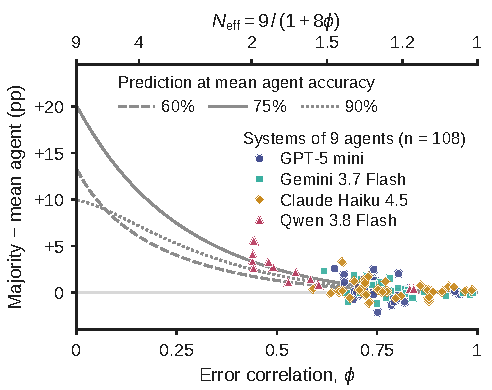
\includegraphics[width=\linewidth]{figures/fig1_teaser_col.pdf}
\caption{\textbf{The benefit of majority voting depends on error correlation.} Majority minus mean agent accuracy versus $\phi$ for $108$ systems of $9$ agents on yes/no items. Gray curves: beta-binomial predictions at mean agent accuracy $60\%$ (dashed), $75\%$ (solid), and $90\%$ (dotted). Top axis: $N_{\mathrm{eff}}=9/(1+8\phi)$. Blue circles: GPT-5 mini; teal squares: Gemini 3.7 Flash; amber diamonds: Claude Haiku 4.5; rose triangles: Qwen 3.8 Flash.}
\label{fig:teaser}
\end{figure}

\begin{itemize}
\item \textbf{Aggregation arithmetic.} Mean agent accuracy and error correlation predict every system's majority accuracy under a beta-binomial model on yes/no items (prediction-error SD: $0.84$~pp). Nine agents of one VLM in the Independent MAS provide $1.17$ to $1.99$ effective independent agents.
\item \textbf{Language prior.} On MedXpertQA-MM, $64.2\%$ to $76.2\%$ of shared wrong answers (at least seven of nine agents wrong) match the majority answer with a blank image.
\item \textbf{Perception versus reasoning.} A perception module writes query-agnostic reports without the question or options; a reasoning module answers from them. Sharing one report increases $\phi$ to $0.800$--$0.990$ relative to own reports. Changing the model lowers $\phi$ most in matched contrasts: $0.470$--$0.492$, compared with $0.033$--$0.060$ for roles.
\item \textbf{Debate and conformity.} In the Decentralized MAS, agents change $41.5\%$ to $100.0\%$ of correct initial minority answers to wrong final answers.
\end{itemize}

\section{Related work}\label{sec:related}

\paragraph{Multi-agent systems in medicine.}
MDAgents adapts collaboration to task complexity \cite{kim2024mdagents}, while MedAgents uses expert analysis and collaborative refinement for zero-shot medical reasoning \cite{tang2024medagents}. Kim et al. identify a capability-saturation threshold for multi-agent gains \cite{kim2026scaling}. Multiagent debate lets model instances revise their responses after reviewing other agents' answers \cite{du2024debate}. MedAgentBoard benchmarks multi-agent collaboration against conventional methods across medical tasks \cite{medagentboard}; Zhu et al. analyze confidence and diversity in debate \cite{demystifying_mad}. We quantify the effective number of independent agents on radiology images and test which shared components account for correlated errors.

\paragraph{Correlated errors and aggregation.}
Dependence limits the precision and value of information from multiple sources \cite{clemen1985limits}. CorrErr measures agreement when language models are both wrong and finds correlated errors across models \cite{correlated2025}. Kish's design effect relates pairwise correlation to effective sample size \cite{kish1965survey}. Pooling independent diagnostic judgments outperforms the best doctor when individual accuracies are similar \cite{kurvers2016pooling}. We predict majority accuracy from Pearson correlation of binary error indicators and mean agent accuracy, then test shared components through matched contrasts.

\paragraph{Language priors and visual reliance in VLMs.}
VQAv2 counters language priors with complementary images \cite{goyal2017vqa}; MMStar emphasizes visual dependency in evaluation \cite{chen2024mmstar}. NaturalBench pairs questions with images that require different answers \cite{li2024naturalbench}, and MMVP tests visual differences missed by CLIP \cite{tong2024eyes}. Medical probing reveals failures on simple diagnosis questions \cite{yan2025worse}, and correct answers can conceal flawed image comprehension \cite{jin2024hidden}. Counterfactual grounding measures reliance on visual evidence \cite{zafar2026see}. Prism decouples VLM perception and reasoning through visual descriptions \cite{qiao2024prism}. We use blank images and query-agnostic reports to measure how language priors and perception contribute to shared errors in multi-agent systems.

\section{Setup}\label{sec:setup}

\begin{figure}[t]
  \centering
  \fbox{\parbox[c][3.6cm][c]{0.95\linewidth}{\centering\small Study design (drawn by the authors)}}
  \caption{\textbf{Controlled comparisons vary visual evidence and shared components.} Systems are single agent, self-consistency, Independent and Decentralized; image manipulations include blank images, reduced resolution, region occlusion and paired images. Query-agnostic reports separate perception from reasoning; outcomes are accuracy, $\phi$ and $N_{\mathrm{eff}}$.}
  \label{fig:design}
\end{figure}

\subsection{Agents and multi-agent systems}
A multi-agent system (MAS) comprises 9 instances of one VLM.
The single agent uses a general-radiologist prompt at temperature 0.3.
Self-consistency is a single-agent baseline with 9 samples of that prompt and majority vote~\cite{wang2023selfconsistency}.
For the Independent MAS, GPT-4.1 nano selects and ranks 9 of 12 subspecialty roles from the question; agents answer separately and majority vote decides.
The Decentralized MAS starts from the same agents' initial answers and allows up to 3 debate rounds, with majority vote over final answers~\cite{kim2026scaling,du2024debate}.
Debate stops at unanimity; peer context is capped at 900 characters.
The nine-agent conditions use temperature 0.7 with seed $100+i$ for agent $i$.
GPT-5 mini accepts neither parameter and uses low reasoning effort.

\subsection{Error correlation and the effective number of agents}
Error correlation $\phi$ is the mean pairwise Pearson correlation of binary error indicators across items; pairs with constant indicators are omitted.
The effective number of independent agents is $N_{\mathrm{eff}}=9/(1+8\phi)$~\cite{kish1965survey}.
On yes/no items, a beta-binomial model predicts majority accuracy from mean agent accuracy $\bar p$ and intraclass correlation $\phi$:
\begin{equation}
  \alpha=\frac{\bar p(1-\phi)}{\phi},\qquad
  \beta=\frac{(1-\bar p)(1-\phi)}{\phi},
\end{equation}
\begin{equation}
  \begin{gathered}
    K\sim\mathrm{BetaBin}(9,\alpha,\beta),\\
    P(\text{majority correct})=P(K\geq 5).
  \end{gathered}
\end{equation}
Multi-agent gain (MAS minus single-agent accuracy) splits into mean agent minus single-agent accuracy plus majority-vote minus mean agent accuracy.

\subsection{Data and models}
Each evaluation set contains 250 items, except SLAKE-pairs (200 pairs).
VQA-RAD and SLAKE use closed yes/no questions~\cite{lau2018vqarad,liu2021slake}; MedXpertQA-MM retains radiologic images only and has 5 options~\cite{zuo2025medxpertqa}.
SLAKE-target adds target and equal-sized, nonoverlapping control boxes.
SLAKE-pairs asks the same question on two images with opposite reference answers, as in NaturalBench and MMVP~\cite{li2024naturalbench,tong2024eyes}.
Proprietary models are GPT-5 mini, Gemini 3.7 Flash, Claude Haiku 4.5 and Qwen 3.8 Flash, accessed through OpenRouter.
Open-weight models are MedGemma 4B, Qwen3-VL 8B, Qwen2-VL 7B, HuatuoGPT-Vision 7B and LLaVA-1.5 7B~\cite{sellergren2025medgemma,bai2025qwen3vl,wang2024qwen2vl,chen2024huatuovision,liu2024llava15}.
Each open-weight item uses one forward pass; answers follow yes/no token probabilities or option-letter probabilities.

\begin{table}[t]
  \centering
  \caption{Experiments and coverage. Main: VQA-RAD, SLAKE and MedXpertQA-MM. Prop.: all four proprietary models for A0/A1 and C role/contrast/model comparisons; the first three otherwise. B crosses perception and reasoning modules.}
  \label{tab:setup}
  \footnotesize
  \setlength{\tabcolsep}{3pt}
  \begin{tabular}{@{}>{\raggedright\arraybackslash}p{0.07\linewidth}>{\raggedright\arraybackslash}p{0.20\linewidth}>{\raggedright\arraybackslash}p{0.48\linewidth}>{\raggedright\arraybackslash}p{0.16\linewidth}@{}}
    \toprule
    Exp. & Data sets & Conditions & Models \\
    \midrule
    A0 & Main & Original images ($\leq$1024 pixels) & Prop. \\
    A1 & Main & Reduced resolution (256, 128 pixels); blank images & Prop. \\
    A2 & SLAKE-target & Target/control occlusion & Prop. \\
    A3 & SLAKE-pairs & Paired original images & Prop. \\
    B & Main & Own/shared query-agnostic reports & $3\times3$ \\
    C & Main & Shared components; in-context examples on VQA-RAD/SLAKE & Prop. \\
    D & All five & A0--A3 image conditions; contrast adjustment & 5 open-weight \\
    \bottomrule
  \end{tabular}
\end{table}

\subsection{Manipulations}
Image manipulations vary visual evidence (\cref{fig:design,tab:setup}); blank images are uniform gray and reduced resolution caps the long side.
Occlusion sensitivity is target minus control answer-change rate~\cite{zeiler2014visualizing}; pair accuracy requires both answers correct.
Perception modules write query-agnostic reports without the question or options; reasoning modules receive the report, question and options without the image~\cite{qiao2024prism}.
Each agent receives a different report in the own-report condition or the same report in the shared-report condition.
Own-report conditions cross all perception and reasoning modules; shared-report conditions use matching models.
The image baseline is self-consistency with the same reasoning module.
Matched contrasts measure $\Delta\phi$ for agents without versus with a shared component: role, contrast adjustment, in-context examples, report, perception module, reasoning module or model.
Contrast adjustment compares original images with gamma correction ($\gamma=0.7$) or contrast-limited adaptive histogram equalization (CLAHE)~\cite{zuiderveld1994clahe}.
In-context examples are shared (the same 3 for all agents) or private (different examples per agent).
Conformity is the share of initially correct agents whose final answer is wrong~\cite{asch1956conformity,demystifying_mad}.
We stratify conformity by initial majority/minority status and agreement with the same agent's blank-image answer.
Protocol details appear in Sec.~\ref{sec:supp-protocol}.

\subsection{Statistics}
Item-bootstrap 95\% confidence intervals (CIs) use 2,000 resamples; $\phi$ uses 500 and matched contrasts use 300.
Resampling retains all responses and matched conditions per item; paired-image analyses resample complete pairs.
Abstentions count as wrong; a sensitivity analysis recomputes $\phi$ on items answered by both agents.

\section{Results}\label{sec:results}

\begin{figure*}[t]
\centering
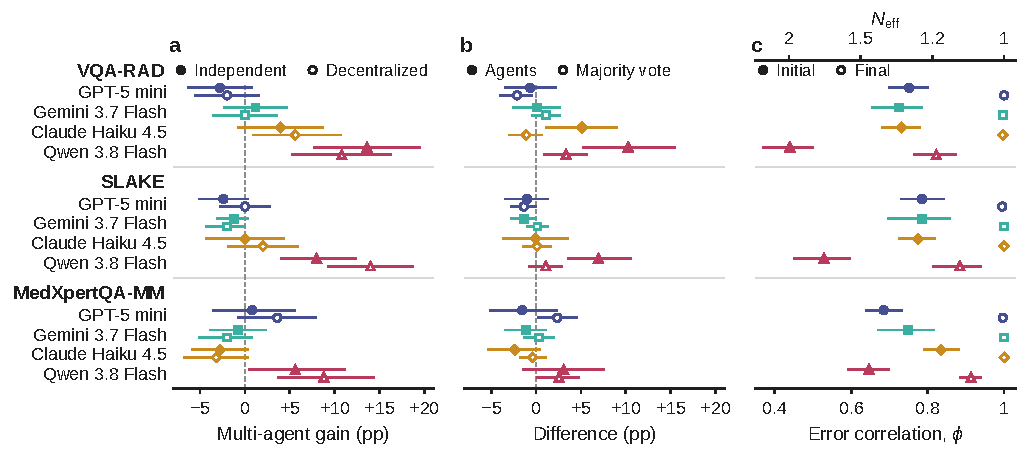
\includegraphics[width=\textwidth]{figures/fig3_panels.pdf}
\caption{\textbf{Nine agents from one VLM are worth fewer than two.}
Rows group models within data sets (250 items each).
(a) Multi-agent gain: Independent (filled) and Decentralized (open) accuracy minus single-agent accuracy.
(b) Independent gain decomposed into mean agent minus single-agent accuracy (Agents, filled) and majority minus mean agent accuracy (Majority vote, open).
(c) Error correlation $\phi$ for initial (filled) and final (open) answers; the top axis gives $N_{\mathrm{eff}}$.
Intervals are paired item-bootstrap 95\% CIs. Model colors as in \cref{fig:teaser}.}
\label{fig:panels}
\end{figure*}

\subsection{Nine agents are worth fewer than two}
Nine agents had an effective number of independent agents of $N_{\mathrm{eff}}=1.17$ to $1.99$ (\cref{fig:panels}).
For GPT-5 mini, Gemini 3.7 Flash, and Claude Haiku 4.5, the range was 1.17 to 1.39; Qwen 3.8 Flash reached 1.46 to 1.99.
The first three models' Independent multi-agent gains ranged from $-2.8$ to 4.0~pp, and their Decentralized gains from $-3.2$ to 5.6~pp.
Claude's Decentralized MAS gained 5.6~pp [0.8, 10.8] on VQA-RAD (Tabs.~S2--S5).

Qwen's larger gains arose mostly before majority voting: mean agent accuracy exceeded single-agent accuracy by 3.1 to 10.3~pp, while voting added 1.1 to 3.3~pp.
Its Independent MAS gained 13.6~pp [7.6, 19.6] on VQA-RAD, 8.0~pp [4.0, 12.4] on SLAKE, and 5.6~pp [0.4, 11.2] on MedXpertQA-MM.
Decentralized gains ranged from 8.8 to 14.0~pp.
For the other models, majority voting changed accuracy by $-2.1$ to 2.4~pp relative to mean agent accuracy (\cref{fig:panels}b).

Debate drove error correlation to 0.995 to 1.000 for GPT-5 mini, Gemini 3.7 Flash and Claude Haiku 4.5 and to 0.822 to 0.913 for Qwen 3.8 Flash (\cref{fig:panels}c).
Final answers were unanimous on 82.4\% to 100.0\% of items, but 8.9\% to 70.0\% of unanimous answers were wrong.

Mean agent accuracy and error correlation predicted majority accuracy with a mean residual of $-0.07$~pp across 108 systems on yes/no items.
The beta-binomial residual SD was 0.84~pp, and the largest absolute residual was 2.59~pp (\cref{fig:teaser,fig:supp-arithmetic}).
Across these systems, majority minus mean agent accuracy ranged from $-2.1$ to 5.6~pp over $\phi=0.44$ to $0.99$.

\begin{figure*}[t]
\centering
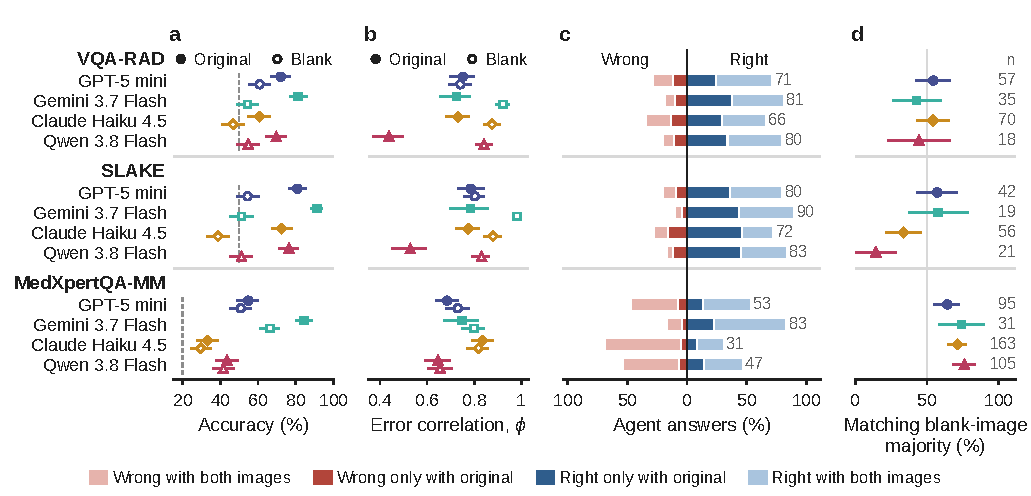
\includegraphics[width=\textwidth]{figures/fig4_prior.pdf}
\caption{\textbf{Most shared wrong answers on MedXpertQA-MM match the blank-image majority.}
(a) Single-agent accuracy with original (filled) and blank (open) images; dashed lines mark chance.
(b) Independent MAS error correlation with each image.
(c) Agent answers cross-tabulated by correctness: wrong with both images, wrong only with original, right only with original, and right with both images; end numbers give original-image accuracy.
(d) Shared wrong answers whose majority matches the blank-image majority; $n$ counts items with at least 7 of 9 agents wrong.
Each data set has 250 items. Intervals are item-bootstrap 95\% CIs. Model colors as in \cref{fig:teaser}.}
\label{fig:prior}
\end{figure*}

\subsection{Agents fall back on the language prior}
On MedXpertQA-MM, 64.2\% to 76.2\% of shared wrong answers matched the blank-image majority (\cref{fig:prior}d).
These items had at least 7 of 9 agents wrong with the original image.
The corresponding shares were 42.9\% to 54.4\% on VQA-RAD and 14.3\% to 57.9\% on SLAKE (Tabs.~S9--S10).

Replacing the image with a uniform gray blank image reduced single-agent accuracy by 11.2 to 26.8~pp on VQA-RAD and 25.2 to 40.0~pp on SLAKE (\cref{fig:prior}a).
On MedXpertQA-MM, losses were 4.0~pp [$-2.0$, 10.0] for GPT-5 mini, 3.6~pp [$-0.4$, 8.0] for Claude, and 2.0~pp [$-4.4$, 8.0] for Qwen.
Gemini lost 18.0~pp [12.0, 23.6] (Tabs.~S6--S8).

With blank images, Gemini, Claude, and Qwen had $\phi=0.841$ to $0.922$ on VQA-RAD and 0.831 to 0.982 on SLAKE (\cref{fig:prior}b).
Original-image ranges were 0.439--0.731 and 0.529--0.785, respectively.
Claude's blank-image correlation remained high after abstentions were excluded: 0.963 on VQA-RAD, 0.931 on SLAKE, and 0.852 on MedXpertQA-MM.
Reduced resolution changed $\phi$ in opposite directions across models: on VQA-RAD, GPT-5 mini fell from 0.752 to 0.644, while Qwen rose from 0.439 to 0.480 (\cref{fig:supp-resolution}).

On VQA-RAD, 24.1\% to 37.3\% of agent answers were correct only with the original image, versus 10.4\% to 13.6\% only with the blank image (\cref{fig:prior}c).
SLAKE shares were 36.3\% to 46.4\% versus 4.4\% to 15.8\%; MedXpertQA-MM shares were 8.1\% to 22.3\% versus 4.4\% to 7.9\%.
On MedXpertQA-MM, 12.3\% to 64.0\% were wrong with both images.

\begin{figure}[t]
\centering
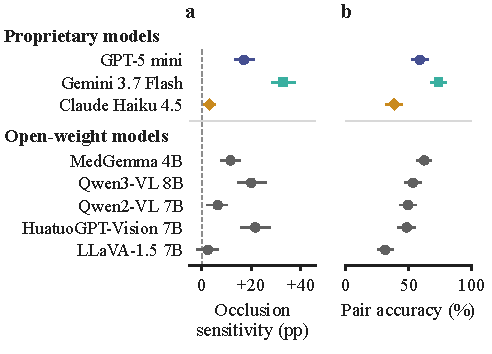
\includegraphics[width=\linewidth]{figures/fig5_region.pdf}
\caption{\textbf{Models differ in their sensitivity to the queried image region.}
(a) Occlusion sensitivity, target minus control answer-change rate, on SLAKE-target (250 items).
(b) Pair accuracy, both answers correct, on SLAKE-pairs (200 pairs with opposite reference answers).
Occlusion estimates average Independent MAS agents for proprietary models; pair accuracy uses single agents.
Open-weight models use one forward pass per item.
Intervals are item-bootstrap 95\% CIs; pairs are resampled intact in (b). Model colors as in \cref{fig:teaser}.}
\label{fig:region}
\end{figure}

\subsection{Models differ in where they look}
Gemini's occlusion sensitivity was 32.9~pp [28.2, 38.0], compared with 17.1~pp [13.2, 21.2] for GPT-5 mini and 3.2~pp [0.8, 5.7] for Claude (\cref{fig:region}a).
This difference subtracts answer changes under an equal-size control occlusion from those under target occlusion.
Open-weight estimates ranged from 2.4 to 21.6~pp; LLaVA-1.5 7B had 2.4~pp [$-2.0$, 6.8] (Tabs.~S11--S12).

Gemini also had the highest proprietary-model pair accuracy: 74.0\% [67.5, 80.0], versus 59.0\% for GPT-5 mini and 38.5\% for Claude (\cref{fig:region}b).
With the same question and opposite reference answers, agents changed their answer between images in 75.0\%, 62.0\%, and 42.5\% of pairs, respectively (Tabs.~S13--S14).
The remaining pairs received identical answers despite the change in reference answer.

\begin{figure*}[t]
\centering
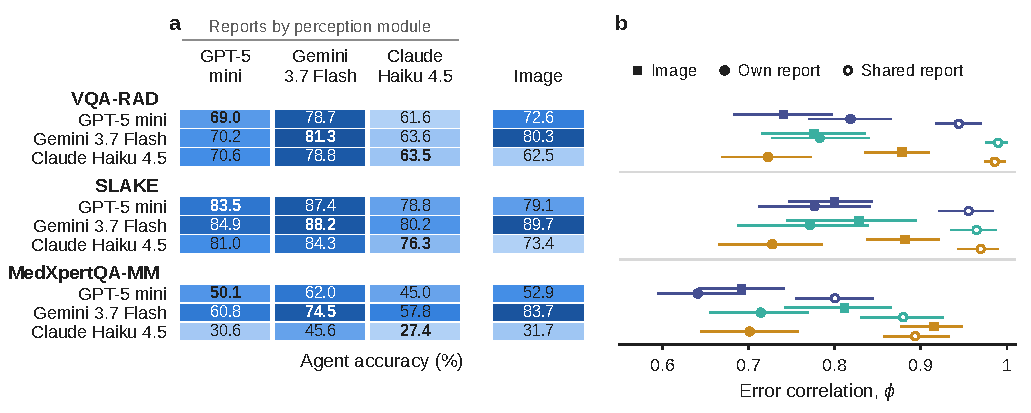
\includegraphics[width=\textwidth]{figures/fig6_report.pdf}
\caption{\textbf{Perception sets accuracy, while sharing a report increases error correlation.}
(a) Agent accuracy with its own query-agnostic report from the column's perception module, or with the image.
Rows identify reasoning modules within data sets (250 items each); shading scales within each data set.
Bold cells use the same model for both modules.
(b) Error correlation among 9 agents: image (filled square), own report (filled circle), and shared report (open circle), with same-model reports.
Intervals are item-bootstrap 95\% CIs. Model colors as in \cref{fig:teaser}.}
\label{fig:report}
\end{figure*}

\subsection{Perception sets accuracy; a shared report sets correlation}
Gemini's query-agnostic reports raised the other reasoning modules' accuracy by 6.1 to 16.3~pp over reading the image (\cref{fig:report}a).
The endpoint effects were 6.1~pp [1.4, 10.9] for GPT-5 mini and 16.3~pp [9.9, 22.6] for Claude on VQA-RAD.
Each agent read its own report without the image.
Across reasoning modules, Gemini reports yielded 78.7\% to 81.3\% accuracy on VQA-RAD and 84.3\% to 88.2\% on SLAKE.
Claude reports lowered the other reasoning modules' accuracy in 5 of 6 cells, by 7.9 to 25.9~pp.
The remaining cell, GPT-5 mini on SLAKE, differed by $-0.4$~pp [$-5.0$, 4.6] (Tabs.~S17--S19).

Under identical Gemini reports on MedXpertQA-MM, accuracy differed by reasoning module: Gemini achieved 74.5\%, GPT-5 mini 62.0\%, and Claude 45.6\%.
With GPT-5 mini reports, their accuracies were 60.8\%, 50.1\%, and 30.6\%, respectively.

The queried target was absent from 26.5\% to 30.8\% of SLAKE reports and from 25.8\% to 47.1\% of reports behind errors.
For Gemini reports, omissions occurred in 26.7\% overall and 33.6\% to 47.1\% of reports behind errors across reasoning modules.

Sharing one report raised $\phi$ to 0.800--0.990, compared with 0.641--0.818 when agents read their own reports from the same model (\cref{fig:report}b).
Both modules were held fixed in this comparison; only the report was shared.

\begin{figure}[t]
\centering
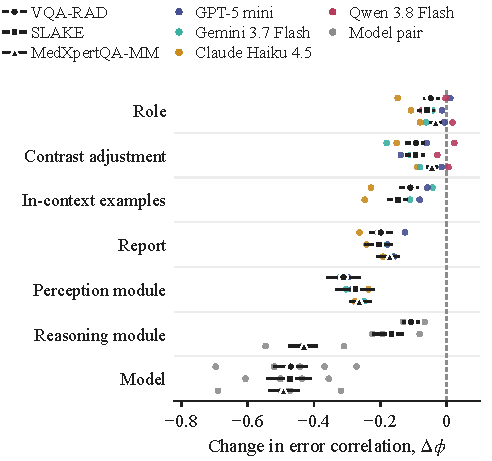
\includegraphics[width=\linewidth]{figures/fig7_contrasts.pdf}
\caption{\textbf{Changing the model reduces error correlation more than changing a component within one model.}
Matched $\Delta\phi$ compares agents differing in the named component with agents sharing it.
Black markers give data-set means: circle, VQA-RAD; square, SLAKE; triangle, MedXpertQA-MM (250 items each).
Colored dots give models; gray dots give model pairs.
In-context examples compare private with shared examples on VQA-RAD and SLAKE.
Report compares own with shared reports; reasoning-module contrasts hold the report fixed.
Intervals are item-bootstrap 95\% CIs. Model colors as in \cref{fig:teaser}.}
\label{fig:contrasts}
\end{figure}

\subsection{What makes two agents err together}
Changing the model produced the largest mean reduction in error correlation, 0.470 to 0.492 across data sets (\cref{fig:contrasts}).
Self-consistency samples of one model had $\phi=0.692$ to $0.915$ for the proprietary models and 0.442 to 0.629 for Qwen (Tabs.~S20--S22).
Mean reductions were 0.033--0.060 for role and 0.045--0.094 for contrast adjustment.
Private in-context examples reduced $\phi$ by 0.110--0.146 relative to shared examples; own reports reduced it by 0.172--0.204 relative to a shared report.
Changing the perception module reduced $\phi$ by 0.263--0.311.

The reasoning-module contrast was largest on MedXpertQA-MM: $\Delta\phi=-0.430$ [$-0.477$, $-0.389$], compared with $-0.263$ for the perception module.
Across data sets, reasoning-module contrasts ranged from $-0.430$ to $-0.108$ under identical reports.
Private examples also separated correlation from accuracy: for Claude on SLAKE, $\phi$ fell from 0.928 to 0.655 with private image examples, while MAS accuracy fell from 70.4\% to 68.8\% (Tabs.~S25--S28).
The additive regression is a secondary summary in Tabs.~S23--S24.

\begin{figure}[t]
\centering
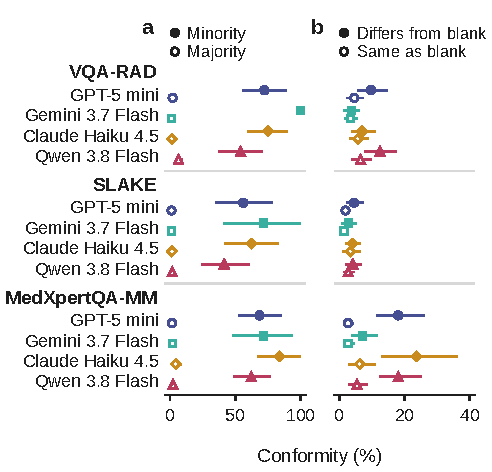
\includegraphics[width=\linewidth]{figures/fig8_discussion.pdf}
\caption{\textbf{Agents change correct minority answers to wrong answers during debate.}
Conformity is the share of initially correct agents whose final answer is wrong in the Decentralized MAS.
(a) Initial minority (filled) versus majority (open).
(b) Initial answer differs from (filled) or matches (open) the same agent's blank-image answer.
Rows group models within data sets (250 items each; 9 agents).
Intervals are item-bootstrap 95\% CIs. Model colors as in \cref{fig:teaser}.}
\label{fig:conformity}
\end{figure}

\subsection{Debate removes correct minority answers}
Agents changed 41.5\% to 100.0\% of correct initial minority answers to wrong answers during debate, versus 1.0\% to 6.5\% of correct majority answers (\cref{fig:conformity}a).
On MedXpertQA-MM, conformity was 7.2\% to 23.6\% when a correct initial answer differed from the same agent's blank-image answer, versus 2.6\% to 6.3\% when it matched (\cref{fig:conformity}b).
Paired differences ranged from 4.6~pp [0.8, 9.0] for Gemini to 17.4~pp [6.4, 29.7] for Claude (Tabs.~S15--S16).
Among correct answers that differed from the blank-image answer, 6.6\% to 23.5\% were initially in the minority on MedXpertQA-MM.

\subsection{Open-weight probes}
Blank images cost four of five open-weight models 16.4 to 19.2~pp on VQA-RAD; LLaVA-1.5 7B lost 2.0~pp (\cref{fig:supp-openweight}).
All five lost 16.0 to 48.8~pp on SLAKE.
On MedXpertQA-MM, original-image accuracy was 20.0\% to 24.4\%, versus 20.0\% to 23.6\% with blank images (Tabs.~S29--S30).
Mean visual reliance, the absolute change in log-odds of yes, ranged from 0.89 to 6.43 on VQA-RAD and 1.40 to 11.23 on SLAKE.
On MedXpertQA-MM, reliance measured by Kullback--Leibler divergence ranged from 0.10 to 0.88.

Error correlation between open-weight models ranged from 0.099 to 0.535 (Tab.~S31).
HuatuoGPT-Vision 7B and LLaVA-1.5 7B share the CLIP ViT-L/14-336 encoder.
Their correlation divided by its maximum given marginal error rates, $\phi/\phi_{\max}$, was 0.213 to 0.451; pairs with different encoders ranged from 0.148 to 0.725.
Proprietary-model shared wrong answers were associated with lower open-weight visual reliance on SLAKE: Spearman $\rho=-0.401$ [$-0.502$, $-0.295$].
It was $-0.048$ [$-0.165$, 0.068] on VQA-RAD and 0.006 [$-0.128$, 0.136] on MedXpertQA-MM.

\section{Discussion}\label{sec:discussion}

Multi-agent systems should be sized by agent accuracy and error dependence, as captured by the beta-binomial analysis (\cref{fig:teaser,fig:supp-arithmetic}). Majority voting has little room to improve decisions when agents fail on the same items. Interventions that reduce $\phi$ should be assessed at matched mean agent accuracy, because majority accuracy depends on both quantities. The gain decomposition separates better agents from better aggregation: a multi-agent gain can reflect a change in mean agent accuracy rather than a benefit from voting.

Shared perception exposes reasoning agents to common omissions, while a shared language prior can favor the same answer without visual support. The report comparisons isolate dependence on common findings (\cref{fig:report}). A query-agnostic report makes the extracted findings available for inspection before reasoning. Its omissions restrict the visual information available to every agent that reads it. On MedXpertQA-MM, agreement with blank-image majorities identifies shared errors that persist without the image (\cref{fig:prior}). Prism's perception--reasoning split makes each module available for model substitution~\cite{qiao2024prism}.

Debate adds peer answers and reasoning to the evidence available to each agent~\cite{du2024debate}. Correct minority answers can be displaced during revision (\cref{fig:conformity}), consistent with conformity in multiagent debate~\cite{demystifying_mad}. Retaining initial answers permits evaluation of which errors communication corrects and which it introduces.

An AI second reading in radiology should be assessed by its complementary errors, with clinical double reading as the reference~\cite{geijer2018double}. The model-substitution contrasts motivate testing a different VLM for this role (\cref{fig:contrasts}). Evaluation should measure joint errors before advice is exchanged: incorrect AI suggestions can alter radiologists' decisions~\cite{dratsch2023automation}.

\paragraph{Limitations.}
This controlled evaluation concerns closed questions from public data sets. Its scope includes neither human readers nor clinical reporting.

\section{Conclusion}

Across the original-image comparisons, nine agents from one VLM represented 1.17 to 1.99 effective independent agents. Shared-report error correlations were $0.800$--$0.990$; $64.2\%$--$76.2\%$ of shared wrong answers matched blank-image majorities on MedXpertQA-MM. Conformity reached $41.5\%$--$100.0\%$ for correct initial minority answers. Changing the model reduced error correlation by $0.470$--$0.492$, the largest reduction among the tested contrasts.

{
    \small
    \bibliographystyle{ieeenat_fullname}
    \bibliography{cvpr_refs}
}

% Supplementary material, compiled with the paper (split before submission)
\clearpage
\setcounter{page}{1}
\maketitlesupplementary
\setcounter{table}{0}\renewcommand{\thetable}{S\arabic{table}}
\setcounter{figure}{0}\renewcommand{\thefigure}{S\arabic{figure}}

\section{Protocol details}\label{sec:supp-protocol}

\subsection{Exclusions and image preparation}
Image eligibility was established before sampling. VQA-RAD used closed yes/no questions from its test split; SLAKE used closed yes/no questions from its English test split. Duplicate image--question combinations were removed from VQA-RAD. For MedXpertQA-MM, GPT-4.1 nano labeled image modality, and Claude Haiku 4.5 also labeled each candidate image as radiologic or not. Drawings and diagrams were excluded, as were photographs, pathology slides, charts and tables. Every attached image had to be radiologic for an item to be eligible.

SLAKE-target required an annotated organ or lesion that was present in the image. It used the English training and test splits and excluded items in the SLAKE evaluation set. The target bounding box was expanded by 10\% on each side and clipped to the image boundaries; the expanded box occupied at most 40\% of the image. An equal-sized control box did not overlap the target and had at least 70\% of its area inside the body. Target and control occlusion used mid-gray fills before resizing. SLAKE-pairs contained the same question with opposite reference answers and allowed at most 5 pairs per question template.

Sampling used stratified shuffling with seed 42. VQA-RAD strata used the reference answer; SLAKE strata also used modality. MedXpertQA-MM strata used body system and medical task. SLAKE-target strata used target type and modality; SLAKE-pairs strata used question template. Yes/no option order was randomized separately for each item from its identifier. Images were resized proportionally, without upsampling, to at most 1024 pixels on the long side. Reduced-resolution conditions capped that side at 256 or 128 pixels. Blank images were uniform gray images of the same dimensions~\cite{zafar2026see}.

\subsection{Agent prompts and sampling}
Role assignment used the question text to select subspecialties. GPT-4.1 nano selected and ranked the 9 most relevant roles from a roster of 12. The roster covered neuroradiology, head and neck, thoracic, cardiovascular, abdominal, genitourinary, musculoskeletal, breast, pediatric, nuclear medicine, interventional and emergency radiology. If fewer than 9 roles were returned, the remaining positions were filled in roster order. Systems of 1, 3 and 9 agents used the first members of this roster and reused their initial answers. The single agent and self-consistency baseline used a general-radiologist prompt, with instructions to reason briefly, step by step, before selecting an answer.

Generation settings were fixed by model and condition. The configuration seed was 1; agent $i$ used seed $100+i$. Where supported, agents in a MAS, debate rounds and perception modules used temperature 0.7; the single agent used 0.3. GPT-5 mini accepted neither seed nor temperature and used low reasoning effort, with separate sampling for its agents. GPT-4.1 nano used temperature 0 for role assignment and modality screening. Decentralized MAS reused Independent MAS initial answers and allowed up to 3 subsequent rounds, with a stop at unanimity. Agents saw peer answers and reasoning; peer context was capped at 900 characters and peer order was shuffled by item and round.

\subsection{Contrast adjustment}
Contrast adjustment assigned different image versions to self-consistency samples. Agents 1--3 saw the original image; agents 4--6 saw a gamma-transformed image with gamma 0.7. Agents 7--9 saw contrast-limited adaptive histogram equalization (CLAHE)~\cite{zuiderveld1994clahe}. CLAHE used a clip limit of 2.0 and an $8\times8$ tile grid on the lightness channel. The corresponding contrast compared agents with different adjustments against self-consistency samples with the original image.

\subsection{In-context example retrieval and selection}
In-context examples came from training images with closed yes/no question--answer pairs. This condition used VQA-RAD and English SLAKE training data and was evaluated on VQA-RAD and SLAKE. The data sets carried no patient identifiers, so exclusions used image identity and similarity. SHA-256 hashes excluded images identical to any test image. For each query, candidates were also excluded within Hamming distance 8 of its 64-bit perceptual hash or at CLIP cosine similarity of at least 0.98.

Retrieval used CLIP ViT-L/14-336 image embeddings~\cite{radford2021clip}. The 27 nearest eligible images were shuffled deterministically by question identifier into 9 groups of 3. In the shared condition, every agent received the first group; in the private condition, agent $i$ received group $i$. For each retrieved image, the question--answer pair with maximal term frequency--inverse document frequency (TF-IDF) cosine similarity to the current question was selected. Examples with images supplied that pair alongside its image. Text-only examples supplied the same question and answer without the image. The single agent also received shared examples with images or as text.

\subsection{Query-agnostic reports and coverage}
Query-agnostic reports separated perception from reasoning~\cite{qiao2024prism}. GPT-5 mini, Gemini 3.7 Flash and Claude Haiku 4.5 each served as a perception module and a reasoning module. Perception modules received neither the question nor its answer options. They were instructed to write at most 120 words that described modality and plane alongside visible anatomy, and to record every abnormal or notable finding with its location.

Each perception module generated 9 reports per image or multi-image set, reused across questions about that image. All reasoning modules received identical reports for a given perception module, image and report index. Reasoning agents received the report, question and options without the image. Each agent used its own report in the own-report condition. All agents used the first report in the shared-report condition, which used matching perception and reasoning modules. Comparisons with direct image input used self-consistency samples from the same reasoning model.

Report coverage on SLAKE used a synonym list based on the supplied organ and lesion labels. A report covered the queried target when it mentioned the target or a listed synonym. Accuracy and error correlation were evaluated by report condition, and errors were separated by target coverage.

\subsection{Open-weight answer probabilities}
Open-weight models used one forward pass per item and condition without sampling. They received the same rendered pixels as the proprietary models. Softmax normalized next-token logits over the answer words yes/no for binary items and over option letters for multiple-option items. Each answer used the highest logit among accepted capitalization and leading-space token variants. The validation comparison that fixed the yes/no readout appears in \cref{tab:supp-validation}.

Visual reliance compared original-image and blank-image probability distributions. On yes/no items it was the absolute change in the log-odds of yes. On MedXpertQA-MM it was the Kullback--Leibler divergence from the original-image distribution to the blank-image distribution. Error correlation between models was also divided by its maximum given their marginal error rates, $\phi_{\max}$. Spearman correlation related shared wrong answers of proprietary models to open-weight visual reliance.

\subsection{Matched contrasts of error correlation}
The primary component analysis used matched differences in mean pairwise error correlation. Each contrast subtracted a condition in which agents shared the named component from one in which they did not:
\begin{itemize}
    \item \textbf{Role:} Independent MAS agents with subspecialty roles minus self-consistency samples with the same general-radiologist prompt.
    \item \textbf{Contrast adjustment:} agents with different contrast adjustments minus self-consistency samples with original images.
    \item \textbf{In-context examples:} agents with private examples minus agents with shared examples, matched by example format, with images or as text.
    \item \textbf{Report:} the own-report condition minus the shared-report condition, with matching perception and reasoning modules.
    \item \textbf{Perception module:} agents that read reports from different perception modules minus agents that read different reports from one perception module, within a reasoning model.
    \item \textbf{Reasoning module:} agents from different reasoning models that read the same report minus agents from one reasoning model that read one shared report.
    \item \textbf{Model:} self-consistency samples from different models minus self-consistency samples from one model.
\end{itemize}

Contrasts were computed within each reasoning model or model pair and then averaged over models or model pairs. For the reasoning-module and model contrasts, the subtracted mean averaged the separate within-model correlations of both models. Cross-model comparisons reused the existing self-consistency responses. Self-consistency error correlation from one model was the reference; it was reported as $\phi$, rather than $\Delta\phi$ (Tab.~S20--S22).

\subsection{Regression and statistical inference}
Ordinary least squares regression supplied an additive secondary summary of pairwise error correlation (Tab.~S23--S24). Predictors indicated components that two agents did not share, including image versus report input. The regression included one intercept per pair of reasoning models. Its coefficients were conditional on the other predictors; the matched contrasts were the primary component analysis.

Error correlation was the mean Pearson correlation of binary error indicators over agent pairs. Pairs with constant error indicators were omitted. For yes/no systems, the beta-binomial majority prediction used mean agent accuracy and error correlation; a majority required at least 5 correct agents out of 9. Shared wrong answers required at least 7 of 9 agents to be wrong. Conformity was the share of initially correct agents whose final answer was wrong~\cite{asch1956conformity,demystifying_mad}. It was stratified by initial majority status and by agreement with the same agent's blank-image answer.

Percentile bootstrap 95\% confidence intervals (CIs) retained all responses and matched conditions for each sampled item. Accuracy intervals used 2,000 item resamples with seed 0; error-correlation intervals used 500. Regression, matched contrasts and initial-to-final correlation comparisons used 300 resamples. Matched contrasts used the same resampled items as the regression. All differences were paired by item; paired-image measures resampled complete pairs. An increase or decrease required a difference CI that excluded zero.

Unparsed answers counted as wrong. These abstentions were reported by condition and mostly reflected refusals to read blank images. A sensitivity analysis recomputed error correlation on items that both agents answered. Pair accuracy required both answers to be correct, with answers compared as option text, yes or no.

\onecolumn
\section{Validation before the main experiments}\label{sec:supp-validation}

Validation fixed generation settings and the open-weight probability readout before the main experiments (\cref{tab:supp-validation}). Accuracy differences in this table use pp.

\begin{table*}[!htbp]
\centering
\caption{\textbf{Validation fixed the settings used in the controlled evaluation.} V1--V6 cover answer parsing, image preparation, retrieval, localization, reports and open-weight readout. CLAHE denotes contrast-limited adaptive histogram equalization; CLIP denotes Contrastive Language--Image Pretraining; CT denotes computed tomography.}
\label{tab:supp-validation}
\footnotesize
\setlength{\tabcolsep}{4pt}
\begin{tabular}{@{}p{0.065\textwidth}p{0.59\textwidth}p{0.30\textwidth}@{}}
\toprule
Check & Result & Setting fixed \\
\midrule
V1 & Single-agent answer parsing was 100\% for all four proprietary models called through OpenRouter. On the same prompt, GPT-5 mini used 256 reasoning tokens at low effort and 2,304 at high effort. & GPT-5 mini used low reasoning effort. \\[3pt]
V2 & Single-agent accuracy relative to the original image over 10 model-by-data-set cells: CLAHE averaged 0.0~pp (range $-6$ to 14); grayscale inversion averaged $-6.6$~pp (range $-12$ to 2). The changes at 256 and 128 pixels were $-1.0$ and $-5.6$~pp. & Inversion exceeded the 5~pp limit. Contrast adjustment used gamma 0.7 for agents 4--6 and CLAHE for agents 7--9. \\[3pt]
V3 & Parsing was 100\% with four images per prompt: the query and three in-context examples. A CLIP threshold of 0.95 removed about 32 similar cases from different patients per query. Radiographs from different patients reached cosines of 0.91 to 0.95. A perceptual hash missed the same CT level and the same patient's chest radiograph (cosine 0.99). & In-context examples used the hash and similarity exclusion rules in \cref{sec:supp-protocol}, with CLIP threshold 0.98. \\[3pt]
V4 & In 20 inspected SLAKE-target cases, the target box covered the queried organ or lesion. The control box did not overlap the target and lay within the body. & Target and control boxes were used as built. \\[3pt]
V5 & Query-agnostic reports had median lengths of 72 to 77 words and a maximum of 109 words. Answer parsing was 100\%. & The report protocol was used as built. \\[3pt]
V6 & With option-letter probabilities, the LLaVA family assigned 96--100\% probability to ``A'' regardless of the image. Pooled accuracy on 100 items, 50 each from VQA-RAD and SLAKE: MedGemma 84\%, HuatuoGPT-Vision 79\%, Qwen3-VL 78\%, Qwen2-VL 74\%, LLaVA-1.5 55\% and LLaVA-Med 53\%. & Binary items used yes/no token logits. LLaVA-Med was excluded by the 55\% pooled-accuracy threshold. \\[3pt]
Runtime & Qwen 3.8 Flash used 250 to 6,400 reasoning tokens and 6 to 77 seconds per call. & Qwen 3.8 Flash used original, reduced-resolution and blank images, self-consistency and contrast adjustment. \\
\bottomrule
\end{tabular}
\end{table*}

\section{Data collection}\label{sec:supp-collection}

All proprietary-model calls used OpenRouter in October 2026. Perception modules generated reports before reasoning-module calls and were instructed to write at most 120 words. GPT-5 mini and Claude Haiku 4.5 each had a median report length of 75 words; Gemini 3.7 Flash had a median of 90. Maximum lengths were 118, 121 and 127 words, respectively. Provider routing and token budgets remained fixed. Transient service failures were retried until every item had a response. The automatic stop at more than 15\% unparsed answers was not applied to blank-image conditions.

% Keep the generated tables at their native width without changing their source.
\section{Detailed results}\label{sec:supp-tables}

Tables S2--S31 report the detailed results with item-bootstrap 95\% CIs. Tables S2--S5 cover original-image systems; S6--S10 cover image resolution and blank-image comparisons. Tables S11--S14 cover occlusion and paired images; S15--S16 cover conformity. Tables S17--S19 cover the perception--reasoning split; S20--S24 cover component contrasts and regression. Tables S25--S28 cover in-context examples; S29--S31 cover open-weight models.

\begingroup
% Keep the longest generated tables within the page height.
\linespread{0.94}\selectfont
% Generated by experiments/cvpr_fig/cvpr_tables.py. Do not edit by hand.

\begin{table*}[!htbp]
\centering
\scriptsize
\setlength{\tabcolsep}{2.4pt}
\caption{Multi-agent systems of 9 agents with original images (250 items per data set): accuracy (\%), multi-agent gain (pp), its split into mean agent minus single agent and majority minus mean agent, error correlation $\phi$ of initial and final answers, $N_{\mathrm{eff}}$, and the final answers of the Decentralized MAS that are unanimous and, among those, wrong (\%).}
\label{tab:s-mas}
\begin{tabular}{llccccccccccccc}
\toprule
\makecell{Data set} & \makecell{Model} & \makecell{Single\\agent} & \makecell{Mean\\agent} & \makecell{Indep.} & \makecell{Decentr.} & \makecell{Indep.\\$-$ single} & \makecell{Decentr.\\$-$ single} & \makecell{Mean agent\\$-$ single} & \makecell{Majority $-$\\mean agent} & \makecell{$\phi$\\initial} & \makecell{$N_{\mathrm{eff}}$} & \makecell{$\phi$\\final} & \makecell{Unani-\\mous} & \makecell{Wrong if\\unanimous} \\
\midrule
VQA-RAD & GPT-5 mini & 72.0 & 71.3 & 69.2 & 70.0 & \makecell{$-$2.8\\{\tiny[$-$6.4, 0.8]}} & \makecell{$-$2.0\\{\tiny[$-$5.6, 1.6]}} & \makecell{$-$0.7\\{\tiny[$-$3.5, 2.2]}} & \makecell{$-$2.1\\{\tiny[$-$4.0, $-$0.4]}} & \makecell{0.752\\{\tiny[0.697, 0.801]}} & 1.28 & \makecell{1.000\\{\tiny[1.000, 1.000]}} & 100.0 & 30.0 \\
 & Gemini 3.7 Flash & 81.2 & 81.3 & 82.4 & 81.2 & \makecell{1.2\\{\tiny[$-$2.4, 4.8]}} & \makecell{0.0\\{\tiny[$-$3.6, 3.6]}} & \makecell{0.1\\{\tiny[$-$2.7, 2.7]}} & \makecell{1.1\\{\tiny[$-$0.5, 2.7]}} & \makecell{0.725\\{\tiny[0.653, 0.785]}} & 1.32 & \makecell{0.997\\{\tiny[0.991, 1.000]}} & 99.6 & 18.9 \\
 & Claude Haiku 4.5 & 60.8 & 65.9 & 64.8 & 66.4 & \makecell{4.0\\{\tiny[$-$0.8, 8.8]}} & \makecell{5.6\\{\tiny[0.8, 10.8]}} & \makecell{5.1\\{\tiny[1.0, 9.1]}} & \makecell{$-$1.1\\{\tiny[$-$3.1, 0.8]}} & \makecell{0.731\\{\tiny[0.678, 0.781]}} & 1.31 & \makecell{0.996\\{\tiny[0.990, 1.000]}} & 99.2 & 33.5 \\
 & Qwen 3.8 Flash & 69.6 & 79.9 & 83.2 & 80.4 & \makecell{13.6\\{\tiny[7.6, 19.6]}} & \makecell{10.8\\{\tiny[5.2, 16.4]}} & \makecell{10.3\\{\tiny[5.2, 15.5]}} & \makecell{3.3\\{\tiny[0.8, 5.8]}} & \makecell{0.439\\{\tiny[0.369, 0.501]}} & 1.99 & \makecell{0.822\\{\tiny[0.762, 0.874]}} & 86.0 & 15.8 \\
\midrule
SLAKE & GPT-5 mini & 80.8 & 79.8 & 78.4 & 80.8 & \makecell{$-$2.4\\{\tiny[$-$5.2, 0.4]}} & \makecell{0.0\\{\tiny[$-$2.8, 2.8]}} & \makecell{$-$1.0\\{\tiny[$-$3.5, 1.3]}} & \makecell{$-$1.4\\{\tiny[$-$2.9, 0.0]}} & \makecell{0.785\\{\tiny[0.729, 0.844]}} & 1.24 & \makecell{0.995\\{\tiny[0.984, 1.000]}} & 99.6 & 18.9 \\
 & Gemini 3.7 Flash & 91.2 & 89.9 & 90.0 & 89.2 & \makecell{$-$1.2\\{\tiny[$-$3.2, 0.4]}} & \makecell{$-$2.0\\{\tiny[$-$4.4, 0.0]}} & \makecell{$-$1.3\\{\tiny[$-$2.8, 0.1]}} & \makecell{0.1\\{\tiny[$-$1.0, 1.3]}} & \makecell{0.785\\{\tiny[0.696, 0.859]}} & 1.24 & \makecell{1.000\\{\tiny[1.000, 1.000]}} & 100.0 & 10.8 \\
 & Claude Haiku 4.5 & 72.4 & 72.3 & 72.4 & 74.4 & \makecell{0.0\\{\tiny[$-$4.4, 4.4]}} & \makecell{2.0\\{\tiny[$-$2.0, 6.0]}} & \makecell{$-$0.1\\{\tiny[$-$3.8, 3.6]}} & \makecell{0.1\\{\tiny[$-$1.6, 1.7]}} & \makecell{0.775\\{\tiny[0.723, 0.821]}} & 1.25 & \makecell{1.000\\{\tiny[1.000, 1.000]}} & 100.0 & 25.6 \\
 & Qwen 3.8 Flash & 76.4 & 83.3 & 84.4 & 90.4 & \makecell{8.0\\{\tiny[4.0, 12.4]}} & \makecell{14.0\\{\tiny[9.2, 18.8]}} & \makecell{6.9\\{\tiny[3.5, 10.6]}} & \makecell{1.1\\{\tiny[$-$0.8, 2.9]}} & \makecell{0.529\\{\tiny[0.448, 0.597]}} & 1.72 & \makecell{0.884\\{\tiny[0.811, 0.940]}} & 94.4 & 8.9 \\
\midrule
MedXpertQA-MM & GPT-5 mini & 54.8 & 53.2 & 55.6 & 58.4 & \makecell{0.8\\{\tiny[$-$3.6, 5.6]}} & \makecell{3.6\\{\tiny[$-$0.8, 8.0]}} & \makecell{$-$1.6\\{\tiny[$-$5.2, 2.4]}} & \makecell{2.4\\{\tiny[0.1, 4.6]}} & \makecell{0.685\\{\tiny[0.636, 0.735]}} & 1.39 & \makecell{0.996\\{\tiny[0.991, 1.000]}} & 98.8 & 41.7 \\
 & Gemini 3.7 Flash & 84.4 & 83.3 & 83.6 & 82.4 & \makecell{$-$0.8\\{\tiny[$-$4.0, 2.4]}} & \makecell{$-$2.0\\{\tiny[$-$5.2, 0.8]}} & \makecell{$-$1.1\\{\tiny[$-$3.5, 1.2]}} & \makecell{0.3\\{\tiny[$-$1.4, 2.0]}} & \makecell{0.749\\{\tiny[0.669, 0.817]}} & 1.29 & \makecell{1.000\\{\tiny[1.000, 1.000]}} & 100.0 & 17.6 \\
 & Claude Haiku 4.5 & 33.2 & 30.8 & 30.4 & 30.0 & \makecell{$-$2.8\\{\tiny[$-$6.0, 0.4]}} & \makecell{$-$3.2\\{\tiny[$-$6.8, 0.4]}} & \makecell{$-$2.4\\{\tiny[$-$5.4, 0.5]}} & \makecell{$-$0.4\\{\tiny[$-$1.9, 1.1]}} & \makecell{0.836\\{\tiny[0.790, 0.882]}} & 1.17 & \makecell{1.000\\{\tiny[1.000, 1.000]}} & 100.0 & 70.0 \\
 & Qwen 3.8 Flash & 43.6 & 46.7 & 49.2 & 52.4 & \makecell{5.6\\{\tiny[0.4, 11.2]}} & \makecell{8.8\\{\tiny[3.6, 14.4]}} & \makecell{3.1\\{\tiny[$-$1.5, 7.6]}} & \makecell{2.5\\{\tiny[0.0, 4.9]}} & \makecell{0.647\\{\tiny[0.591, 0.701]}} & 1.46 & \makecell{0.913\\{\tiny[0.883, 0.941]}} & 82.4 & 42.7 \\
\bottomrule
\end{tabular}
\end{table*}

\begin{table*}[!htbp]
\centering
\scriptsize
\setlength{\tabcolsep}{3.2pt}
\caption{Reduced resolution and blank images: single-agent accuracy (\%) and error correlation $\phi$ of the Independent MAS of 9 agents with original images ($\le$1024 pixels), images capped at 256 and 128 pixels, and blank images (uniform gray, same size); single-agent accuracy lost with the blank image (pp); unparsed answers with the blank image (\%) and $\phi$ recomputed on items both agents answered.}
\label{tab:s-resolution}
\begin{tabular}{llccccccccccc}
\toprule
\makecell{Data set} & \makecell{Model} & \makecell{Acc.\\original} & \makecell{Acc.\\256 px} & \makecell{Acc.\\128 px} & \makecell{Acc.\\blank} & \makecell{$\phi$\\original} & \makecell{$\phi$\\256 px} & \makecell{$\phi$\\128 px} & \makecell{$\phi$\\blank} & \makecell{Original $-$\\blank} & \makecell{Unparsed,\\blank} & \makecell{$\phi$ blank,\\answered} \\
\midrule
VQA-RAD & GPT-5 mini & \makecell{72.0\\{\tiny[66.4, 77.2]}} & \makecell{74.0\\{\tiny[68.8, 79.2]}} & \makecell{72.8\\{\tiny[67.2, 78.0]}} & \makecell{60.8\\{\tiny[54.8, 66.4]}} & \makecell{0.752\\{\tiny[0.697, 0.801]}} & \makecell{0.694\\{\tiny[0.636, 0.751]}} & \makecell{0.644\\{\tiny[0.586, 0.703]}} & \makecell{0.742\\{\tiny[0.689, 0.789]}} & \makecell{11.2\\{\tiny[4.0, 18.4]}} & 0.0 & -- \\
 & Gemini 3.7 Flash & \makecell{81.2\\{\tiny[76.4, 86.0]}} & \makecell{83.6\\{\tiny[78.8, 88.0]}} & \makecell{77.6\\{\tiny[72.4, 82.4]}} & \makecell{54.4\\{\tiny[48.4, 60.4]}} & \makecell{0.725\\{\tiny[0.653, 0.785]}} & \makecell{0.726\\{\tiny[0.646, 0.793]}} & \makecell{0.749\\{\tiny[0.698, 0.804]}} & \makecell{0.922\\{\tiny[0.889, 0.951]}} & \makecell{26.8\\{\tiny[18.8, 35.2]}} & 0.0 & -- \\
 & Claude Haiku 4.5 & \makecell{60.8\\{\tiny[54.4, 66.8]}} & \makecell{63.2\\{\tiny[57.2, 69.2]}} & \makecell{65.2\\{\tiny[59.2, 70.8]}} & \makecell{46.8\\{\tiny[40.8, 52.8]}} & \makecell{0.731\\{\tiny[0.678, 0.781]}} & \makecell{0.706\\{\tiny[0.651, 0.756]}} & \makecell{0.591\\{\tiny[0.539, 0.650]}} & \makecell{0.876\\{\tiny[0.840, 0.911]}} & \makecell{14.0\\{\tiny[6.0, 22.0]}} & 10.4 & \makecell{0.963\\{\tiny[0.942, 0.982]}} \\
 & Qwen 3.8 Flash & \makecell{69.6\\{\tiny[64.0, 75.2]}} & \makecell{67.6\\{\tiny[61.6, 73.2]}} & \makecell{72.0\\{\tiny[66.4, 77.6]}} & \makecell{54.8\\{\tiny[48.4, 60.8]}} & \makecell{0.439\\{\tiny[0.369, 0.501]}} & \makecell{0.442\\{\tiny[0.377, 0.501]}} & \makecell{0.480\\{\tiny[0.415, 0.541]}} & \makecell{0.841\\{\tiny[0.805, 0.879]}} & \makecell{14.8\\{\tiny[6.4, 23.2]}} & 0.1 & -- \\
\midrule
SLAKE & GPT-5 mini & \makecell{80.8\\{\tiny[76.0, 85.6]}} & \makecell{78.8\\{\tiny[73.6, 83.6]}} & \makecell{75.2\\{\tiny[70.0, 80.4]}} & \makecell{54.4\\{\tiny[48.4, 60.8]}} & \makecell{0.785\\{\tiny[0.729, 0.844]}} & \makecell{0.792\\{\tiny[0.741, 0.845]}} & \makecell{0.709\\{\tiny[0.645, 0.761]}} & \makecell{0.802\\{\tiny[0.755, 0.845]}} & \makecell{26.4\\{\tiny[18.8, 33.2]}} & 0.0 & -- \\
 & Gemini 3.7 Flash & \makecell{91.2\\{\tiny[87.6, 94.4]}} & \makecell{91.2\\{\tiny[87.6, 94.8]}} & \makecell{85.2\\{\tiny[80.8, 89.2]}} & \makecell{51.2\\{\tiny[44.8, 57.6]}} & \makecell{0.785\\{\tiny[0.696, 0.859]}} & \makecell{0.803\\{\tiny[0.716, 0.869]}} & \makecell{0.820\\{\tiny[0.753, 0.872]}} & \makecell{0.982\\{\tiny[0.968, 0.994]}} & \makecell{40.0\\{\tiny[33.2, 46.8]}} & 0.0 & -- \\
 & Claude Haiku 4.5 & \makecell{72.4\\{\tiny[67.2, 78.0]}} & \makecell{73.6\\{\tiny[68.0, 78.8]}} & \makecell{70.0\\{\tiny[64.4, 75.6]}} & \makecell{38.8\\{\tiny[32.8, 44.8]}} & \makecell{0.775\\{\tiny[0.723, 0.821]}} & \makecell{0.752\\{\tiny[0.695, 0.811]}} & \makecell{0.718\\{\tiny[0.664, 0.768]}} & \makecell{0.879\\{\tiny[0.841, 0.915]}} & \makecell{33.6\\{\tiny[24.0, 42.8]}} & 4.3 & \makecell{0.931\\{\tiny[0.901, 0.956]}} \\
 & Qwen 3.8 Flash & \makecell{76.4\\{\tiny[70.8, 81.2]}} & \makecell{74.8\\{\tiny[69.2, 80.8]}} & \makecell{79.2\\{\tiny[74.4, 84.0]}} & \makecell{51.2\\{\tiny[44.8, 57.2]}} & \makecell{0.529\\{\tiny[0.448, 0.597]}} & \makecell{0.547\\{\tiny[0.479, 0.607]}} & \makecell{0.490\\{\tiny[0.408, 0.560]}} & \makecell{0.831\\{\tiny[0.788, 0.866]}} & \makecell{25.2\\{\tiny[16.4, 33.6]}} & 0.0 & -- \\
\midrule
MedXpertQA-MM & GPT-5 mini & \makecell{54.8\\{\tiny[48.8, 60.4]}} & \makecell{50.4\\{\tiny[44.4, 56.8]}} & \makecell{50.8\\{\tiny[44.8, 56.8]}} & \makecell{50.8\\{\tiny[44.8, 56.4]}} & \makecell{0.685\\{\tiny[0.636, 0.735]}} & \makecell{0.690\\{\tiny[0.637, 0.739]}} & \makecell{0.700\\{\tiny[0.652, 0.752]}} & \makecell{0.730\\{\tiny[0.679, 0.780]}} & \makecell{4.0\\{\tiny[$-$2.0, 10.0]}} & 0.0 & -- \\
 & Gemini 3.7 Flash & \makecell{84.4\\{\tiny[79.6, 88.8]}} & \makecell{80.4\\{\tiny[75.2, 85.2]}} & \makecell{78.4\\{\tiny[73.2, 83.2]}} & \makecell{66.4\\{\tiny[60.8, 71.6]}} & \makecell{0.749\\{\tiny[0.669, 0.817]}} & \makecell{0.762\\{\tiny[0.698, 0.823]}} & \makecell{0.784\\{\tiny[0.715, 0.841]}} & \makecell{0.799\\{\tiny[0.748, 0.844]}} & \makecell{18.0\\{\tiny[12.0, 23.6]}} & 0.0 & -- \\
 & Claude Haiku 4.5 & \makecell{33.2\\{\tiny[27.6, 38.8]}} & \makecell{32.0\\{\tiny[26.4, 37.6]}} & \makecell{32.0\\{\tiny[26.4, 37.6]}} & \makecell{29.6\\{\tiny[24.0, 35.2]}} & \makecell{0.836\\{\tiny[0.790, 0.882]}} & \makecell{0.821\\{\tiny[0.776, 0.868]}} & \makecell{0.840\\{\tiny[0.795, 0.881]}} & \makecell{0.818\\{\tiny[0.765, 0.861]}} & \makecell{3.6\\{\tiny[$-$0.4, 8.0]}} & 14.8 & \makecell{0.852\\{\tiny[0.803, 0.891]}} \\
 & Qwen 3.8 Flash & \makecell{43.6\\{\tiny[37.6, 49.6]}} & \makecell{40.8\\{\tiny[34.8, 47.2]}} & \makecell{43.2\\{\tiny[37.2, 49.6]}} & \makecell{41.6\\{\tiny[35.6, 47.6]}} & \makecell{0.647\\{\tiny[0.591, 0.701]}} & \makecell{0.630\\{\tiny[0.573, 0.688]}} & \makecell{0.609\\{\tiny[0.556, 0.667]}} & \makecell{0.656\\{\tiny[0.602, 0.709]}} & \makecell{2.0\\{\tiny[$-$4.4, 8.0]}} & 0.5 & -- \\
\bottomrule
\end{tabular}
\end{table*}

\begin{table*}[!htbp]
\centering
\scriptsize
\setlength{\tabcolsep}{3.2pt}
\caption{Agent answers of the Independent MAS of 9 cross-tabulated by correctness with the original and the blank image (\% of answers), and shared wrong answers (at least 7 of 9 agents wrong) whose majority answer matches the blank-image majority.}
\label{tab:s-prior}
\begin{tabular}{llcccccc}
\toprule
\makecell{Data set} & \makecell{Model} & \makecell{Right with\\both} & \makecell{Right only\\with original} & \makecell{Wrong only\\with original} & \makecell{Wrong with\\both} & \makecell{Shared wrong\\answers ($n$)} & \makecell{Matching blank-\\image majority (\%)} \\
\midrule
VQA-RAD & GPT-5 mini & 47.2 & 24.1 & 12.0 & 16.7 & 57 & \makecell{54.4\\{\tiny[42.1, 66.7]}} \\
 & Gemini 3.7 Flash & 44.0 & 37.3 & 10.4 & 8.3 & 35 & \makecell{42.9\\{\tiny[25.7, 60.0]}} \\
 & Claude Haiku 4.5 & 36.6 & 29.3 & 13.6 & 20.5 & 70 & \makecell{54.3\\{\tiny[42.9, 65.7]}} \\
 & Qwen 3.8 Flash & 46.0 & 33.9 & 10.8 & 9.3 & 18 & \makecell{44.4\\{\tiny[22.2, 66.7]}} \\
\midrule
SLAKE & GPT-5 mini & 43.5 & 36.3 & 9.5 & 10.7 & 42 & \makecell{57.1\\{\tiny[42.9, 71.4]}} \\
 & Gemini 3.7 Flash & 46.7 & 43.2 & 4.4 & 5.8 & 19 & \makecell{57.9\\{\tiny[36.8, 78.9]}} \\
 & Claude Haiku 4.5 & 25.9 & 46.4 & 15.8 & 11.9 & 56 & \makecell{33.9\\{\tiny[21.4, 46.4]}} \\
 & Qwen 3.8 Flash & 38.5 & 44.8 & 12.0 & 4.7 & 21 & \makecell{14.3\\{\tiny[0.0, 28.6]}} \\
\midrule
MedXpertQA-MM & GPT-5 mini & 39.7 & 13.5 & 7.9 & 38.9 & 95 & \makecell{64.2\\{\tiny[54.7, 72.7]}} \\
 & Gemini 3.7 Flash & 61.0 & 22.3 & 4.4 & 12.3 & 31 & \makecell{74.2\\{\tiny[58.1, 90.3]}} \\
 & Claude Haiku 4.5 & 22.7 & 8.1 & 5.2 & 64.0 & 163 & \makecell{71.2\\{\tiny[64.4, 77.9]}} \\
 & Qwen 3.8 Flash & 32.9 & 13.8 & 7.0 & 46.4 & 105 & \makecell{76.2\\{\tiny[67.6, 83.8]}} \\
\bottomrule
\end{tabular}
\end{table*}

\begin{table}[!htbp]
\centering
\scriptsize
\setlength{\tabcolsep}{3.2pt}
\caption{Region occlusion (SLAKE-target, 250 items) and paired images (SLAKE-pairs, 200 pairs). Answer-change rates under target and control occlusion (\%; proprietary models: agents of the Independent MAS of 9; open-weight models: one forward pass), occlusion sensitivity (target minus control, pp), pair accuracy and the share of pairs answered differently (\%; single agent).}
\label{tab:s-region}
\begin{tabular}{llccccc}
\toprule
\makecell{Model} & \makecell{} & \makecell{Target\\change} & \makecell{Control\\change} & \makecell{Occlusion\\sensitivity} & \makecell{Pair\\accuracy} & \makecell{Answers\\differ} \\
\midrule
GPT-5 mini & proprietary & \makecell{23.5\\{\tiny[19.7, 27.6]}} & \makecell{6.4\\{\tiny[4.7, 8.4]}} & \makecell{17.1\\{\tiny[13.2, 21.2]}} & \makecell{59.0\\{\tiny[52.0, 65.5]}} & \makecell{62.0\\{\tiny[55.5, 68.5]}} \\
Gemini 3.7 Flash & proprietary & \makecell{36.4\\{\tiny[31.6, 41.4]}} & \makecell{3.6\\{\tiny[2.4, 4.9]}} & \makecell{32.9\\{\tiny[28.2, 38.0]}} & \makecell{74.0\\{\tiny[67.5, 80.0]}} & \makecell{75.0\\{\tiny[69.0, 81.0]}} \\
Claude Haiku 4.5 & proprietary & \makecell{10.7\\{\tiny[8.2, 13.6]}} & \makecell{7.5\\{\tiny[5.5, 9.6]}} & \makecell{3.2\\{\tiny[0.8, 5.7]}} & \makecell{38.5\\{\tiny[31.5, 45.0]}} & \makecell{42.5\\{\tiny[35.5, 49.5]}} \\
\midrule
MedGemma 4B & open-weight & \makecell{13.2\\{\tiny[9.2, 17.6]}} & \makecell{1.6\\{\tiny[0.4, 3.2]}} & \makecell{11.6\\{\tiny[7.6, 15.6]}} & \makecell{62.5\\{\tiny[56.0, 68.5]}} & \makecell{63.5\\{\tiny[57.0, 69.5]}} \\
Qwen3-VL 8B & open-weight & \makecell{23.6\\{\tiny[18.4, 28.8]}} & \makecell{3.6\\{\tiny[1.6, 6.0]}} & \makecell{20.0\\{\tiny[14.4, 26.0]}} & \makecell{53.5\\{\tiny[46.5, 60.5]}} & \makecell{56.5\\{\tiny[49.5, 63.0]}} \\
Qwen2-VL 7B & open-weight & \makecell{11.2\\{\tiny[7.6, 15.2]}} & \makecell{4.8\\{\tiny[2.4, 7.6]}} & \makecell{6.4\\{\tiny[2.0, 10.4]}} & \makecell{49.5\\{\tiny[42.5, 56.0]}} & \makecell{53.5\\{\tiny[46.5, 60.0]}} \\
\midrule
HuatuoGPT-Vision 7B & open-weight & \makecell{28.0\\{\tiny[22.4, 34.0]}} & \makecell{6.4\\{\tiny[3.6, 9.6]}} & \makecell{21.6\\{\tiny[15.6, 28.0]}} & \makecell{48.5\\{\tiny[41.5, 55.5]}} & \makecell{53.0\\{\tiny[46.0, 60.0]}} \\
LLaVA-1.5 7B & open-weight & \makecell{12.8\\{\tiny[8.8, 17.2]}} & \makecell{10.4\\{\tiny[6.8, 14.4]}} & \makecell{2.4\\{\tiny[$-$2.0, 6.8]}} & \makecell{31.5\\{\tiny[25.5, 38.0]}} & \makecell{39.5\\{\tiny[33.0, 46.5]}} \\
\bottomrule
\end{tabular}
\end{table}

\begin{table*}[!htbp]
\centering
\scriptsize
\setlength{\tabcolsep}{3.2pt}
\caption{Conformity in the Decentralized MAS of 9 agents: share of correct initial answers that are wrong after debate (\%), for answers in the initial minority or majority, and for answers that differ from or match the same agent's blank-image answer (difference in pp); share of correct initial answers in the initial minority among those that differ from or match the blank-image answer (\%).}
\label{tab:s-conformity}
\begin{tabular}{llccccccc}
\toprule
\makecell{Data set} & \makecell{Model} & \makecell{Initial\\minority} & \makecell{Initial\\majority} & \makecell{Differs\\from blank} & \makecell{Matches\\blank} & \makecell{Difference} & \makecell{In minority,\\differs} & \makecell{In minority,\\matches} \\
\midrule
VQA-RAD & GPT-5 mini & \makecell{72.3\\{\tiny[55.2, 88.9]}} & \makecell{1.9\\{\tiny[0.4, 3.8]}} & \makecell{9.8\\{\tiny[5.5, 14.9]}} & \makecell{4.6\\{\tiny[2.3, 7.4]}} & \makecell{5.1\\{\tiny[0.4, 10.4]}} & \makecell{11.2\\{\tiny[6.8, 16.4]}} & \makecell{3.8\\{\tiny[2.0, 5.9]}} \\
 & Gemini 3.7 Flash & \makecell{100.0\\{\tiny[100.0, 100.0]}} & \makecell{1.0\\{\tiny[0.0, 2.3]}} & \makecell{3.7\\{\tiny[1.4, 6.2]}} & \makecell{3.4\\{\tiny[1.6, 5.7]}} & \makecell{0.3\\{\tiny[$-$2.9, 3.3]}} & \makecell{2.5\\{\tiny[0.8, 4.5]}} & \makecell{2.6\\{\tiny[1.1, 4.5]}} \\
 & Claude Haiku 4.5 & \makecell{75.0\\{\tiny[59.2, 89.7]}} & \makecell{1.4\\{\tiny[0.0, 3.2]}} & \makecell{7.1\\{\tiny[3.9, 11.0]}} & \makecell{5.7\\{\tiny[3.1, 8.9]}} & \makecell{1.4\\{\tiny[$-$2.9, 5.9]}} & \makecell{8.5\\{\tiny[5.2, 12.8]}} & \makecell{5.3\\{\tiny[3.0, 8.0]}} \\
 & Qwen 3.8 Flash & \makecell{54.1\\{\tiny[37.4, 70.6]}} & \makecell{6.5\\{\tiny[3.9, 9.4]}} & \makecell{12.5\\{\tiny[7.8, 17.7]}} & \makecell{6.6\\{\tiny[3.8, 9.8]}} & \makecell{5.9\\{\tiny[0.6, 11.5]}} & \makecell{6.2\\{\tiny[3.4, 9.4]}} & \makecell{4.9\\{\tiny[2.6, 7.7]}} \\
\midrule
SLAKE & GPT-5 mini & \makecell{56.1\\{\tiny[34.9, 78.8]}} & \makecell{1.1\\{\tiny[0.0, 2.5]}} & \makecell{4.5\\{\tiny[2.1, 7.3]}} & \makecell{1.9\\{\tiny[0.8, 3.3]}} & \makecell{2.6\\{\tiny[0.3, 5.2]}} & \makecell{4.0\\{\tiny[2.1, 6.4]}} & \makecell{3.4\\{\tiny[1.7, 5.5]}} \\
 & Gemini 3.7 Flash & \makecell{71.4\\{\tiny[41.2, 100.0]}} & \makecell{1.2\\{\tiny[0.2, 2.4]}} & \makecell{2.9\\{\tiny[0.7, 5.3]}} & \makecell{1.4\\{\tiny[0.3, 2.9]}} & \makecell{1.5\\{\tiny[$-$1.1, 4.2]}} & \makecell{1.8\\{\tiny[0.5, 3.5]}} & \makecell{1.0\\{\tiny[0.3, 2.1]}} \\
 & Claude Haiku 4.5 & \makecell{62.5\\{\tiny[41.4, 83.0]}} & \makecell{1.4\\{\tiny[0.3, 2.9]}} & \makecell{4.0\\{\tiny[1.9, 6.7]}} & \makecell{3.4\\{\tiny[1.1, 6.4]}} & \makecell{0.6\\{\tiny[$-$3.3, 4.1]}} & \makecell{3.4\\{\tiny[1.8, 5.7]}} & \makecell{4.8\\{\tiny[2.0, 8.3]}} \\
 & Qwen 3.8 Flash & \makecell{41.5\\{\tiny[23.7, 61.2]}} & \makecell{1.8\\{\tiny[0.7, 3.1]}} & \makecell{4.2\\{\tiny[2.0, 6.9]}} & \makecell{2.8\\{\tiny[1.3, 4.6]}} & \makecell{1.4\\{\tiny[$-$1.4, 4.6]}} & \makecell{3.4\\{\tiny[1.6, 5.5]}} & \makecell{5.5\\{\tiny[3.3, 8.5]}} \\
\midrule
MedXpertQA-MM & GPT-5 mini & \makecell{68.5\\{\tiny[52.6, 85.3]}} & \makecell{1.4\\{\tiny[0.0, 3.4]}} & \makecell{18.1\\{\tiny[11.5, 26.1]}} & \makecell{2.7\\{\tiny[1.4, 4.3]}} & \makecell{15.4\\{\tiny[9.6, 23.1]}} & \makecell{20.1\\{\tiny[13.3, 28.4]}} & \makecell{3.5\\{\tiny[1.8, 5.5]}} \\
 & Gemini 3.7 Flash & \makecell{71.7\\{\tiny[48.0, 93.9]}} & \makecell{1.9\\{\tiny[0.6, 3.5]}} & \makecell{7.2\\{\tiny[3.7, 11.6]}} & \makecell{2.6\\{\tiny[1.2, 4.5]}} & \makecell{4.6\\{\tiny[0.8, 9.0]}} & \makecell{6.6\\{\tiny[3.3, 11.0]}} & \makecell{1.5\\{\tiny[0.6, 2.6]}} \\
 & Claude Haiku 4.5 & \makecell{83.9\\{\tiny[67.3, 100.0]}} & \makecell{4.4\\{\tiny[0.9, 9.1]}} & \makecell{23.6\\{\tiny[12.8, 36.3]}} & \makecell{6.3\\{\tiny[2.9, 11.1]}} & \makecell{17.4\\{\tiny[6.4, 29.7]}} & \makecell{19.8\\{\tiny[11.1, 31.0]}} & \makecell{3.9\\{\tiny[1.7, 6.9]}} \\
 & Qwen 3.8 Flash & \makecell{62.2\\{\tiny[48.6, 76.7]}} & \makecell{2.4\\{\tiny[0.7, 4.5]}} & \makecell{18.1\\{\tiny[12.3, 25.1]}} & \makecell{5.4\\{\tiny[2.9, 8.5]}} & \makecell{12.7\\{\tiny[6.6, 19.8]}} & \makecell{23.5\\{\tiny[16.3, 32.1]}} & \makecell{6.2\\{\tiny[3.6, 9.4]}} \\
\bottomrule
\end{tabular}
\end{table*}

\begin{table*}[!htbp]
\centering
\scriptsize
\setlength{\tabcolsep}{2.0pt}
\caption{Perception and reasoning. (a) Mean agent accuracy (\%) of each reasoning module when every agent reads its own query-agnostic report from the named perception module, or reads the image (self-consistency samples of the reasoning module); the change from the image (pp); error correlation $\phi$ of 9 agents reading the image, their own reports and one shared report (perception and reasoning module the same model). (b) SLAKE: reports that do not mention the queried target, among all reports and among the reports behind wrong answers (\%).}
\label{tab:s-report}
{\footnotesize (a) Accuracy and error correlation}\par\smallskip
\begin{tabular}{llcccccccccc}
\toprule
\makecell{Data set} & \makecell{Reasoning\\module} & \makecell{Reports by\\GPT-5 mini} & \makecell{Reports by\\Gemini} & \makecell{Reports by\\Claude} & \makecell{Image} & \makecell{GPT-5 mini reports\\$-$ image} & \makecell{Gemini reports\\$-$ image} & \makecell{Claude reports\\$-$ image} & \makecell{$\phi$\\image} & \makecell{$\phi$ own\\reports} & \makecell{$\phi$ shared\\report} \\
\midrule
VQA-RAD & GPT-5 mini & \makecell{69.0\\{\tiny[63.7, 73.9]}} & \makecell{78.7\\{\tiny[74.1, 82.8]}} & \makecell{61.6\\{\tiny[56.4, 66.7]}} & \makecell{72.6\\{\tiny[67.6, 77.3]}} & \makecell{$-$3.6\\{\tiny[$-$8.4, 1.4]}} & \makecell{6.1\\{\tiny[1.4, 10.9]}} & \makecell{$-$10.9\\{\tiny[$-$16.8, $-$5.0]}} & \makecell{0.741\\{\tiny[0.683, 0.797]}} & \makecell{0.818\\{\tiny[0.770, 0.866]}} & \makecell{0.944\\{\tiny[0.917, 0.970]}} \\
 & Gemini 3.7 Flash & \makecell{70.2\\{\tiny[64.6, 75.2]}} & \makecell{81.3\\{\tiny[76.9, 85.4]}} & \makecell{63.6\\{\tiny[58.4, 68.6]}} & \makecell{80.3\\{\tiny[75.6, 84.5]}} & \makecell{$-$10.1\\{\tiny[$-$16.1, $-$4.0]}} & \makecell{1.0\\{\tiny[$-$4.0, 6.0]}} & \makecell{$-$16.7\\{\tiny[$-$23.4, $-$10.1]}} & \makecell{0.776\\{\tiny[0.715, 0.836]}} & \makecell{0.783\\{\tiny[0.727, 0.841]}} & \makecell{0.990\\{\tiny[0.975, 1.000]}} \\
 & Claude Haiku 4.5 & \makecell{70.6\\{\tiny[65.4, 75.6]}} & \makecell{78.8\\{\tiny[74.2, 83.1]}} & \makecell{63.5\\{\tiny[58.1, 68.4]}} & \makecell{62.5\\{\tiny[56.7, 68.0]}} & \makecell{8.1\\{\tiny[1.4, 14.9]}} & \makecell{16.3\\{\tiny[9.9, 22.6]}} & \makecell{0.9\\{\tiny[$-$5.3, 6.8]}} & \makecell{0.878\\{\tiny[0.835, 0.911]}} & \makecell{0.723\\{\tiny[0.668, 0.773]}} & \makecell{0.986\\{\tiny[0.973, 0.998]}} \\
\midrule
SLAKE & GPT-5 mini & \makecell{83.5\\{\tiny[79.3, 87.5]}} & \makecell{87.4\\{\tiny[83.7, 90.9]}} & \makecell{78.8\\{\tiny[74.3, 82.9]}} & \makecell{79.1\\{\tiny[74.5, 83.6]}} & \makecell{4.4\\{\tiny[0.9, 8.2]}} & \makecell{8.3\\{\tiny[4.4, 12.4]}} & \makecell{$-$0.4\\{\tiny[$-$5.0, 4.6]}} & \makecell{0.800\\{\tiny[0.746, 0.844]}} & \makecell{0.777\\{\tiny[0.711, 0.842]}} & \makecell{0.955\\{\tiny[0.921, 0.985]}} \\
 & Gemini 3.7 Flash & \makecell{84.9\\{\tiny[81.0, 88.7]}} & \makecell{88.2\\{\tiny[84.6, 91.6]}} & \makecell{80.2\\{\tiny[76.0, 84.4]}} & \makecell{89.7\\{\tiny[86.3, 93.1]}} & \makecell{$-$4.8\\{\tiny[$-$8.5, $-$1.3]}} & \makecell{$-$1.6\\{\tiny[$-$4.0, 1.2]}} & \makecell{$-$9.5\\{\tiny[$-$13.9, $-$4.9]}} & \makecell{0.828\\{\tiny[0.744, 0.895]}} & \makecell{0.771\\{\tiny[0.687, 0.840]}} & \makecell{0.965\\{\tiny[0.934, 0.988]}} \\
 & Claude Haiku 4.5 & \makecell{81.0\\{\tiny[76.8, 85.1]}} & \makecell{84.3\\{\tiny[80.4, 88.1]}} & \makecell{76.3\\{\tiny[71.8, 80.8]}} & \makecell{73.4\\{\tiny[68.1, 78.5]}} & \makecell{7.6\\{\tiny[3.1, 12.1]}} & \makecell{10.9\\{\tiny[6.4, 15.7]}} & \makecell{2.9\\{\tiny[$-$1.6, 7.3]}} & \makecell{0.882\\{\tiny[0.838, 0.922]}} & \makecell{0.728\\{\tiny[0.665, 0.785]}} & \makecell{0.969\\{\tiny[0.943, 0.990]}} \\
\midrule
MedXpertQA-MM & GPT-5 mini & \makecell{50.1\\{\tiny[45.0, 55.2]}} & \makecell{62.0\\{\tiny[56.7, 67.2]}} & \makecell{45.0\\{\tiny[40.1, 49.9]}} & \makecell{52.9\\{\tiny[47.7, 58.0]}} & \makecell{$-$2.8\\{\tiny[$-$6.9, 1.0]}} & \makecell{9.1\\{\tiny[3.4, 14.4]}} & \makecell{$-$7.9\\{\tiny[$-$12.7, $-$3.2]}} & \makecell{0.692\\{\tiny[0.642, 0.742]}} & \makecell{0.641\\{\tiny[0.595, 0.696]}} & \makecell{0.800\\{\tiny[0.755, 0.845]}} \\
 & Gemini 3.7 Flash & \makecell{60.8\\{\tiny[55.6, 65.9]}} & \makecell{74.5\\{\tiny[69.6, 79.1]}} & \makecell{57.8\\{\tiny[52.7, 62.7]}} & \makecell{83.7\\{\tiny[79.4, 87.8]}} & \makecell{$-$22.9\\{\tiny[$-$28.4, $-$17.5]}} & \makecell{$-$9.2\\{\tiny[$-$13.3, $-$5.2]}} & \makecell{$-$25.9\\{\tiny[$-$31.2, $-$20.4]}} & \makecell{0.811\\{\tiny[0.742, 0.866]}} & \makecell{0.715\\{\tiny[0.654, 0.770]}} & \makecell{0.880\\{\tiny[0.831, 0.927]}} \\
 & Claude Haiku 4.5 & \makecell{30.6\\{\tiny[25.6, 35.7]}} & \makecell{45.6\\{\tiny[40.0, 50.9]}} & \makecell{27.4\\{\tiny[22.6, 32.2]}} & \makecell{31.7\\{\tiny[26.3, 37.3]}} & \makecell{$-$1.1\\{\tiny[$-$5.9, 3.6]}} & \makecell{13.8\\{\tiny[7.8, 19.5]}} & \makecell{$-$4.4\\{\tiny[$-$9.0, $-$0.0]}} & \makecell{0.915\\{\tiny[0.876, 0.949]}} & \makecell{0.701\\{\tiny[0.644, 0.758]}} & \makecell{0.893\\{\tiny[0.857, 0.933]}} \\
\bottomrule
\end{tabular}
\par\medskip
{\footnotesize (b) Target absent from the report, SLAKE}\par\smallskip
\begin{tabular}{lcccccc}
\toprule
\makecell{Reasoning\\module} & \makecell{GPT-5 mini reports,\\all} & \makecell{GPT-5 mini reports,\\behind errors} & \makecell{Gemini reports,\\all} & \makecell{Gemini reports,\\behind errors} & \makecell{Claude reports,\\all} & \makecell{Claude reports,\\behind errors} \\
\midrule
GPT-5 mini & 26.5 & 29.8 & 26.7 & 36.4 & 30.8 & 40.6 \\
Gemini 3.7 Flash & 26.5 & 25.8 & 26.7 & 33.6 & 30.8 & 39.1 \\
Claude Haiku 4.5 & 26.5 & 29.9 & 26.7 & 47.1 & 30.8 & 42.9 \\
\bottomrule
\end{tabular}
\end{table*}

\begin{table}[!htbp]
\centering
\scriptsize
\setlength{\tabcolsep}{3.2pt}
\caption{Matched contrasts of error correlation: $\phi$ of two self-consistency agents of one model, and the mean change $\Delta\phi$ over models (or model pairs) when two agents do not share the named component. In-context examples were run on VQA-RAD and SLAKE.}
\label{tab:s-contrasts}
\begin{tabular}{lccc}
\toprule
\makecell{} & \makecell{VQA-RAD} & \makecell{SLAKE} & \makecell{MedXpertQA-MM} \\
\midrule
Self-consistency $\phi$, GPT-5 mini & \makecell{0.741\\{\tiny[0.676, 0.792]}} & \makecell{0.800\\{\tiny[0.751, 0.847]}} & \makecell{0.692\\{\tiny[0.642, 0.739]}} \\
Self-consistency $\phi$, Gemini 3.7 Flash & \makecell{0.776\\{\tiny[0.714, 0.825]}} & \makecell{0.828\\{\tiny[0.754, 0.906]}} & \makecell{0.811\\{\tiny[0.743, 0.863]}} \\
Self-consistency $\phi$, Claude Haiku 4.5 & \makecell{0.878\\{\tiny[0.836, 0.918]}} & \makecell{0.882\\{\tiny[0.836, 0.921]}} & \makecell{0.915\\{\tiny[0.885, 0.949]}} \\
Self-consistency $\phi$, Qwen 3.8 Flash & \makecell{0.442\\{\tiny[0.378, 0.504]}} & \makecell{0.604\\{\tiny[0.530, 0.666]}} & \makecell{0.629\\{\tiny[0.570, 0.685]}} \\
\midrule
$\Delta\phi$, Role & \makecell{$-$0.048\\{\tiny[$-$0.071, $-$0.023]}} & \makecell{$-$0.060\\{\tiny[$-$0.087, $-$0.036]}} & \makecell{$-$0.033\\{\tiny[$-$0.051, $-$0.014]}} \\
$\Delta\phi$, Contrast adjustment & \makecell{$-$0.092\\{\tiny[$-$0.123, $-$0.068]}} & \makecell{$-$0.094\\{\tiny[$-$0.123, $-$0.066]}} & \makecell{$-$0.045\\{\tiny[$-$0.062, $-$0.027]}} \\
$\Delta\phi$, In-context examples & \makecell{$-$0.110\\{\tiny[$-$0.142, $-$0.084]}} & \makecell{$-$0.146\\{\tiny[$-$0.179, $-$0.117]}} & -- \\
$\Delta\phi$, Report & \makecell{$-$0.199\\{\tiny[$-$0.233, $-$0.164]}} & \makecell{$-$0.204\\{\tiny[$-$0.247, $-$0.162]}} & \makecell{$-$0.172\\{\tiny[$-$0.211, $-$0.142]}} \\
\midrule
$\Delta\phi$, Perception module & \makecell{$-$0.311\\{\tiny[$-$0.362, $-$0.260]}} & \makecell{$-$0.275\\{\tiny[$-$0.334, $-$0.218]}} & \makecell{$-$0.263\\{\tiny[$-$0.294, $-$0.227]}} \\
$\Delta\phi$, Reasoning module & \makecell{$-$0.108\\{\tiny[$-$0.132, $-$0.083]}} & \makecell{$-$0.167\\{\tiny[$-$0.222, $-$0.129]}} & \makecell{$-$0.430\\{\tiny[$-$0.477, $-$0.389]}} \\
$\Delta\phi$, Model & \makecell{$-$0.470\\{\tiny[$-$0.522, $-$0.421]}} & \makecell{$-$0.473\\{\tiny[$-$0.544, $-$0.406]}} & \makecell{$-$0.492\\{\tiny[$-$0.536, $-$0.445]}} \\
\bottomrule
\end{tabular}
\end{table}

\begin{table*}[!htbp]
\centering
\scriptsize
\setlength{\tabcolsep}{3.2pt}
\caption{Additive regression of pairwise error correlation on the components two agents do not share (one intercept per pair of reasoning modules), a secondary summary of Tab.~\ref{tab:s-contrasts}.}
\label{tab:s-regression}
\begin{tabular}{lccccccc}
\toprule
\makecell{Data set} & \makecell{Perception\\module} & \makecell{Image vs\\report} & \makecell{Contrast\\adjustment} & \makecell{Role} & \makecell{In-context\\examples} & \makecell{Report} & \makecell{Reasoning\\module} \\
\midrule
VQA-RAD & \makecell{$-$0.247\\{\tiny[$-$0.283, $-$0.210]}} & \makecell{$-$0.123\\{\tiny[$-$0.173, $-$0.078]}} & \makecell{$-$0.023\\{\tiny[$-$0.036, $-$0.009]}} & \makecell{$-$0.006\\{\tiny[$-$0.016, 0.005]}} & \makecell{$-$0.026\\{\tiny[$-$0.043, $-$0.011]}} & \makecell{0.150\\{\tiny[0.092, 0.218]}} & \makecell{$-$0.026\\{\tiny[$-$0.045, $-$0.004]}} \\
SLAKE & \makecell{$-$0.193\\{\tiny[$-$0.232, $-$0.146]}} & \makecell{$-$0.094\\{\tiny[$-$0.135, $-$0.060]}} & \makecell{$-$0.017\\{\tiny[$-$0.032, $-$0.003]}} & \makecell{$-$0.004\\{\tiny[$-$0.015, 0.006]}} & \makecell{$-$0.040\\{\tiny[$-$0.053, $-$0.028]}} & \makecell{0.009\\{\tiny[$-$0.051, 0.059]}} & \makecell{$-$0.124\\{\tiny[$-$0.168, $-$0.086]}} \\
MedXpertQA-MM & \makecell{$-$0.160\\{\tiny[$-$0.187, $-$0.131]}} & \makecell{$-$0.099\\{\tiny[$-$0.127, $-$0.071]}} & \makecell{$-$0.012\\{\tiny[$-$0.021, $-$0.003]}} & \makecell{$-$0.009\\{\tiny[$-$0.017, $-$0.002]}} & -- & \makecell{$-$0.066\\{\tiny[$-$0.104, $-$0.022]}} & \makecell{$-$0.194\\{\tiny[$-$0.228, $-$0.164]}} \\
\bottomrule
\end{tabular}
\end{table*}

\begin{table*}[!htbp]
\centering
\scriptsize
\setlength{\tabcolsep}{3.2pt}
\caption{In-context examples (VQA-RAD and SLAKE): single-agent accuracy, accuracy of the Independent MAS of 9 agents (\%) and its error correlation $\phi$ without examples, with shared examples (the same 3 for every agent) and with private examples (different examples per agent), given with their images or as text. The single agent received shared examples only.}
\label{tab:s-icl}
\begin{tabular}{lllccccc}
\toprule
\makecell{Data set} & \makecell{Model} & \makecell{} & \makecell{None} & \makecell{Shared,\\images} & \makecell{Private,\\images} & \makecell{Shared,\\text} & \makecell{Private,\\text} \\
\midrule
VQA-RAD & GPT-5 mini & Single agent & \makecell{72.0\\{\tiny[66.4, 77.2]}} & \makecell{73.6\\{\tiny[68.0, 78.8]}} & -- & \makecell{75.6\\{\tiny[70.0, 80.4]}} & -- \\
 &  & MAS accuracy & \makecell{73.6\\{\tiny[68.0, 78.8]}} & \makecell{74.8\\{\tiny[69.6, 80.4]}} & \makecell{75.2\\{\tiny[69.6, 80.4]}} & \makecell{76.4\\{\tiny[71.2, 81.6]}} & \makecell{74.8\\{\tiny[69.6, 80.0]}} \\
 &  & $\phi$ & \makecell{0.741\\{\tiny[0.683, 0.797]}} & \makecell{0.751\\{\tiny[0.694, 0.799]}} & \makecell{0.668\\{\tiny[0.608, 0.723]}} & \makecell{0.737\\{\tiny[0.681, 0.792]}} & \makecell{0.703\\{\tiny[0.637, 0.759]}} \\
\midrule
 & Gemini 3.7 Flash & Single agent & \makecell{81.2\\{\tiny[76.4, 86.0]}} & \makecell{82.4\\{\tiny[77.2, 87.2]}} & -- & \makecell{83.6\\{\tiny[78.8, 88.0]}} & -- \\
 &  & MAS accuracy & \makecell{80.4\\{\tiny[75.2, 84.8]}} & \makecell{82.8\\{\tiny[78.4, 87.2]}} & \makecell{82.0\\{\tiny[77.2, 86.4]}} & \makecell{84.4\\{\tiny[80.0, 88.8]}} & \makecell{84.4\\{\tiny[79.6, 88.8]}} \\
 &  & $\phi$ & \makecell{0.776\\{\tiny[0.715, 0.836]}} & \makecell{0.708\\{\tiny[0.640, 0.772]}} & \makecell{0.673\\{\tiny[0.599, 0.744]}} & \makecell{0.743\\{\tiny[0.658, 0.816]}} & \makecell{0.692\\{\tiny[0.618, 0.763]}} \\
\midrule
 & Claude Haiku 4.5 & Single agent & \makecell{60.8\\{\tiny[54.4, 66.8]}} & \makecell{68.8\\{\tiny[63.2, 74.0]}} & -- & \makecell{61.2\\{\tiny[54.8, 67.2]}} & -- \\
 &  & MAS accuracy & \makecell{62.0\\{\tiny[55.6, 68.0]}} & \makecell{65.2\\{\tiny[58.8, 71.2]}} & \makecell{64.4\\{\tiny[58.8, 70.0]}} & \makecell{62.4\\{\tiny[56.0, 68.4]}} & \makecell{62.4\\{\tiny[56.0, 68.0]}} \\
 &  & $\phi$ & \makecell{0.878\\{\tiny[0.835, 0.911]}} & \makecell{0.890\\{\tiny[0.849, 0.928]}} & \makecell{0.664\\{\tiny[0.612, 0.713]}} & \makecell{0.912\\{\tiny[0.878, 0.942]}} & \makecell{0.681\\{\tiny[0.630, 0.739]}} \\
\midrule
SLAKE & GPT-5 mini & Single agent & \makecell{80.8\\{\tiny[76.0, 85.6]}} & \makecell{79.2\\{\tiny[74.4, 84.0]}} & -- & \makecell{81.6\\{\tiny[76.8, 86.4]}} & -- \\
 &  & MAS accuracy & \makecell{78.4\\{\tiny[73.2, 83.6]}} & \makecell{81.6\\{\tiny[76.8, 86.4]}} & \makecell{84.0\\{\tiny[79.2, 88.4]}} & \makecell{82.0\\{\tiny[77.2, 86.8]}} & \makecell{81.6\\{\tiny[76.8, 86.4]}} \\
 &  & $\phi$ & \makecell{0.800\\{\tiny[0.746, 0.844]}} & \makecell{0.741\\{\tiny[0.667, 0.807]}} & \makecell{0.667\\{\tiny[0.600, 0.737]}} & \makecell{0.780\\{\tiny[0.718, 0.842]}} & \makecell{0.690\\{\tiny[0.620, 0.752]}} \\
\midrule
 & Gemini 3.7 Flash & Single agent & \makecell{91.2\\{\tiny[87.6, 94.4]}} & \makecell{89.2\\{\tiny[85.2, 92.8]}} & -- & \makecell{90.8\\{\tiny[87.2, 94.4]}} & -- \\
 &  & MAS accuracy & \makecell{90.0\\{\tiny[86.4, 93.6]}} & \makecell{89.2\\{\tiny[85.6, 92.8]}} & \makecell{90.4\\{\tiny[86.8, 93.6]}} & \makecell{90.4\\{\tiny[86.4, 94.0]}} & \makecell{92.0\\{\tiny[88.8, 95.2]}} \\
 &  & $\phi$ & \makecell{0.828\\{\tiny[0.744, 0.895]}} & \makecell{0.836\\{\tiny[0.761, 0.894]}} & \makecell{0.722\\{\tiny[0.629, 0.797]}} & \makecell{0.823\\{\tiny[0.725, 0.891]}} & \makecell{0.716\\{\tiny[0.599, 0.804]}} \\
\midrule
 & Claude Haiku 4.5 & Single agent & \makecell{72.4\\{\tiny[67.2, 78.0]}} & \makecell{67.6\\{\tiny[62.0, 73.2]}} & -- & \makecell{76.8\\{\tiny[71.6, 82.0]}} & -- \\
 &  & MAS accuracy & \makecell{73.6\\{\tiny[68.0, 79.2]}} & \makecell{70.4\\{\tiny[64.8, 76.0]}} & \makecell{68.8\\{\tiny[62.8, 74.8]}} & \makecell{78.0\\{\tiny[73.2, 83.2]}} & \makecell{78.0\\{\tiny[73.2, 82.8]}} \\
 &  & $\phi$ & \makecell{0.882\\{\tiny[0.838, 0.922]}} & \makecell{0.928\\{\tiny[0.894, 0.955]}} & \makecell{0.655\\{\tiny[0.608, 0.708]}} & \makecell{0.941\\{\tiny[0.907, 0.970]}} & \makecell{0.720\\{\tiny[0.657, 0.779]}} \\
\bottomrule
\end{tabular}
\end{table*}

\begin{table*}[!htbp]
\centering
\scriptsize
\setlength{\tabcolsep}{3.2pt}
\caption{Open-weight models (one forward pass per item). (a) Accuracy (\%) with original, blank, 256-pixel and 128-pixel images, and mean visual reliance ($|\Delta$ log-odds of yes$|$ between original and blank image on yes/no items; Kullback--Leibler divergence on MedXpertQA-MM). (b) Error correlation $\phi$ between two models and $\phi/\phi_{\max}$, its ratio to the maximum given the two marginal error rates; HuatuoGPT-Vision 7B and LLaVA-1.5 7B share the CLIP ViT-L/14-336 encoder.}
\label{tab:s-openweight}
{\footnotesize (a) Accuracy and visual reliance}\par\smallskip
\begin{tabular}{llccccc}
\toprule
\makecell{Model} & \makecell{Data set} & \makecell{Original} & \makecell{Blank} & \makecell{256 px} & \makecell{128 px} & \makecell{Visual\\reliance} \\
\midrule
MedGemma 4B & VQA-RAD & \makecell{80.0\\{\tiny[75.2, 84.8]}} & \makecell{60.8\\{\tiny[54.8, 66.8]}} & \makecell{80.4\\{\tiny[75.6, 85.2]}} & \makecell{76.0\\{\tiny[71.2, 81.2]}} & \makecell{6.43\\{\tiny[5.71, 7.17]}} \\
 & SLAKE & \makecell{88.8\\{\tiny[85.2, 92.4]}} & \makecell{40.0\\{\tiny[34.0, 46.4]}} & \makecell{86.8\\{\tiny[82.8, 91.2]}} & \makecell{84.0\\{\tiny[79.6, 88.4]}} & \makecell{11.23\\{\tiny[10.58, 11.95]}} \\
 & MedXpertQA-MM & \makecell{22.0\\{\tiny[16.8, 27.2]}} & \makecell{23.2\\{\tiny[18.0, 28.4]}} & \makecell{22.4\\{\tiny[17.2, 27.6]}} & \makecell{22.4\\{\tiny[17.2, 27.6]}} & \makecell{0.88\\{\tiny[0.65, 1.13]}} \\
\midrule
Qwen3-VL 8B & VQA-RAD & \makecell{74.0\\{\tiny[68.4, 79.2]}} & \makecell{57.6\\{\tiny[51.6, 63.6]}} & \makecell{70.0\\{\tiny[64.0, 75.6]}} & \makecell{68.8\\{\tiny[62.8, 74.4]}} & \makecell{5.98\\{\tiny[5.36, 6.61]}} \\
 & SLAKE & \makecell{79.2\\{\tiny[74.0, 84.4]}} & \makecell{43.6\\{\tiny[37.6, 49.6]}} & \makecell{83.6\\{\tiny[78.8, 88.0]}} & \makecell{81.2\\{\tiny[76.4, 86.0]}} & \makecell{9.72\\{\tiny[8.95, 10.55]}} \\
 & MedXpertQA-MM & \makecell{24.4\\{\tiny[19.2, 30.0]}} & \makecell{23.6\\{\tiny[18.8, 28.8]}} & \makecell{25.6\\{\tiny[20.4, 31.2]}} & \makecell{25.2\\{\tiny[20.0, 30.4]}} & \makecell{0.72\\{\tiny[0.55, 0.93]}} \\
\midrule
Qwen2-VL 7B & VQA-RAD & \makecell{76.8\\{\tiny[71.6, 82.0]}} & \makecell{58.8\\{\tiny[53.2, 64.4]}} & \makecell{73.6\\{\tiny[68.4, 78.8]}} & \makecell{76.4\\{\tiny[70.8, 81.6]}} & \makecell{1.49\\{\tiny[1.33, 1.64]}} \\
 & SLAKE & \makecell{78.0\\{\tiny[73.2, 83.2]}} & \makecell{43.2\\{\tiny[36.8, 49.6]}} & \makecell{72.8\\{\tiny[67.6, 78.4]}} & \makecell{68.0\\{\tiny[62.4, 74.0]}} & \makecell{2.44\\{\tiny[2.21, 2.66]}} \\
 & MedXpertQA-MM & \makecell{20.8\\{\tiny[16.0, 26.0]}} & \makecell{21.6\\{\tiny[16.8, 26.8]}} & \makecell{21.2\\{\tiny[16.4, 26.4]}} & \makecell{21.2\\{\tiny[16.4, 26.4]}} & \makecell{0.11\\{\tiny[0.08, 0.14]}} \\
\midrule
HuatuoGPT-Vision 7B & VQA-RAD & \makecell{74.8\\{\tiny[69.6, 80.0]}} & \makecell{56.4\\{\tiny[50.4, 62.4]}} & \makecell{77.2\\{\tiny[72.0, 82.4]}} & \makecell{75.6\\{\tiny[70.4, 80.8]}} & \makecell{0.89\\{\tiny[0.77, 1.01]}} \\
 & SLAKE & \makecell{76.8\\{\tiny[72.0, 82.0]}} & \makecell{50.8\\{\tiny[44.4, 57.2]}} & \makecell{76.0\\{\tiny[70.8, 81.2]}} & \makecell{76.0\\{\tiny[70.8, 81.6]}} & \makecell{1.84\\{\tiny[1.66, 2.03]}} \\
 & MedXpertQA-MM & \makecell{20.0\\{\tiny[15.2, 25.2]}} & \makecell{20.0\\{\tiny[15.2, 25.2]}} & \makecell{19.6\\{\tiny[15.2, 24.4]}} & \makecell{20.4\\{\tiny[15.6, 25.2]}} & \makecell{0.10\\{\tiny[0.07, 0.13]}} \\
\midrule
LLaVA-1.5 7B & VQA-RAD & \makecell{56.0\\{\tiny[49.6, 62.0]}} & \makecell{54.0\\{\tiny[48.0, 60.0]}} & \makecell{56.4\\{\tiny[50.4, 62.4]}} & \makecell{56.0\\{\tiny[49.6, 62.0]}} & \makecell{1.10\\{\tiny[1.02, 1.18]}} \\
 & SLAKE & \makecell{66.0\\{\tiny[59.6, 72.0]}} & \makecell{50.0\\{\tiny[43.6, 56.4]}} & \makecell{66.4\\{\tiny[60.4, 72.4]}} & \makecell{66.0\\{\tiny[60.4, 72.0]}} & \makecell{1.40\\{\tiny[1.29, 1.52]}} \\
 & MedXpertQA-MM & \makecell{21.2\\{\tiny[16.4, 26.4]}} & \makecell{20.4\\{\tiny[15.6, 25.6]}} & \makecell{21.2\\{\tiny[16.4, 26.4]}} & \makecell{20.8\\{\tiny[16.0, 25.6]}} & \makecell{0.10\\{\tiny[0.07, 0.14]}} \\
\bottomrule
\end{tabular}
\par\medskip
{\footnotesize (b) Error correlation between models}\par\smallskip
\begin{tabular}{lccccccc}
\toprule
\makecell{Model pair} & \makecell{Shared\\encoder} & \makecell{VQA-RAD,\\$\phi$} & \makecell{VQA-RAD,\\$\phi/\phi_{\max}$} & \makecell{SLAKE,\\$\phi$} & \makecell{SLAKE,\\$\phi/\phi_{\max}$} & \makecell{MedXpertQA-MM,\\$\phi$} & \makecell{MedXpertQA-MM,\\$\phi/\phi_{\max}$} \\
\midrule
MedGemma 4B -- Qwen3-VL 8B &  & 0.365 & 0.432 & 0.224 & 0.324 & 0.238 & 0.254 \\
MedGemma 4B -- Qwen2-VL 7B &  & 0.294 & 0.323 & 0.485 & 0.725 & 0.227 & 0.236 \\
MedGemma 4B -- HuatuoGPT-Vision 7B &  & 0.332 & 0.385 & 0.316 & 0.488 & 0.338 & 0.359 \\
MedGemma 4B -- LLaVA-1.5 7B &  & 0.181 & 0.321 & 0.227 & 0.459 & 0.244 & 0.250 \\
Qwen3-VL 8B -- Qwen2-VL 7B &  & 0.322 & 0.348 & 0.418 & 0.433 & 0.282 & 0.313 \\
Qwen3-VL 8B -- HuatuoGPT-Vision 7B &  & 0.412 & 0.421 & 0.535 & 0.574 & 0.275 & 0.312 \\
Qwen3-VL 8B -- LLaVA-1.5 7B &  & 0.099 & 0.148 & 0.360 & 0.505 & 0.161 & 0.176 \\
Qwen2-VL 7B -- HuatuoGPT-Vision 7B &  & 0.227 & 0.239 & 0.371 & 0.385 & 0.507 & 0.520 \\
Qwen2-VL 7B -- LLaVA-1.5 7B &  & 0.162 & 0.261 & 0.373 & 0.504 & 0.192 & 0.195 \\
HuatuoGPT-Vision 7B -- LLaVA-1.5 7B & yes & 0.172 & 0.263 & 0.346 & 0.451 & 0.205 & 0.213 \\
\bottomrule
\end{tabular}
\end{table*}

\endgroup

\clearpage
\section{Supplementary figures}\label{sec:supp-figures}

\begin{figure*}[!htbp]
\centering
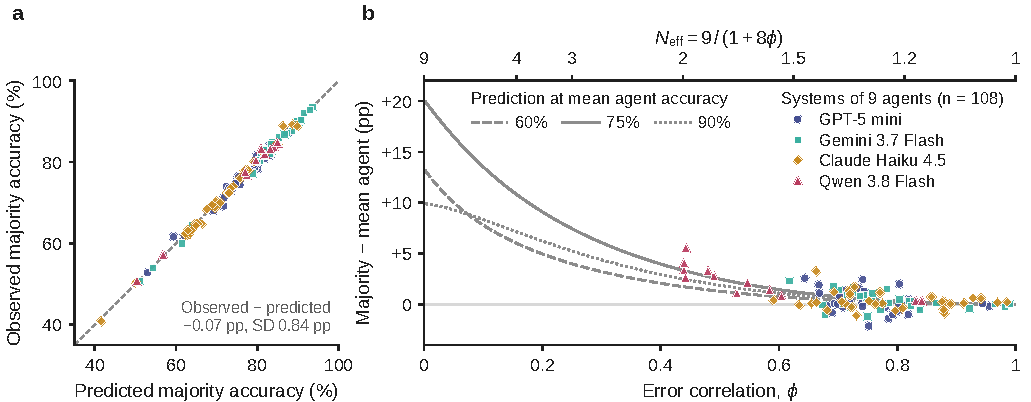
\includegraphics[width=\textwidth]{figures/fig1_teaser_full.pdf}
\caption{\textbf{Mean agent accuracy and error correlation predict majority accuracy on yes/no items.} (a) Observed versus beta-binomial predicted majority accuracy for 108 systems of 9 agents; the dashed diagonal marks equality. Observed minus predicted accuracy averaged $-0.07$~pp, with standard deviation (SD) 0.84~pp. (b) Majority minus mean agent accuracy against error correlation $\phi$; gray curves give predictions at mean agent accuracy 60\% (dashed), 75\% (solid) and 90\% (dotted). The top axis gives $N_{\mathrm{eff}}=9/(1+8\phi)$. The systems used VQA-RAD, SLAKE and SLAKE-target (250 items each), and SLAKE-pairs (200 pairs). Model colors as in Fig.~1.}
\label{fig:supp-arithmetic}
\end{figure*}

\begin{figure*}[!htbp]
\centering
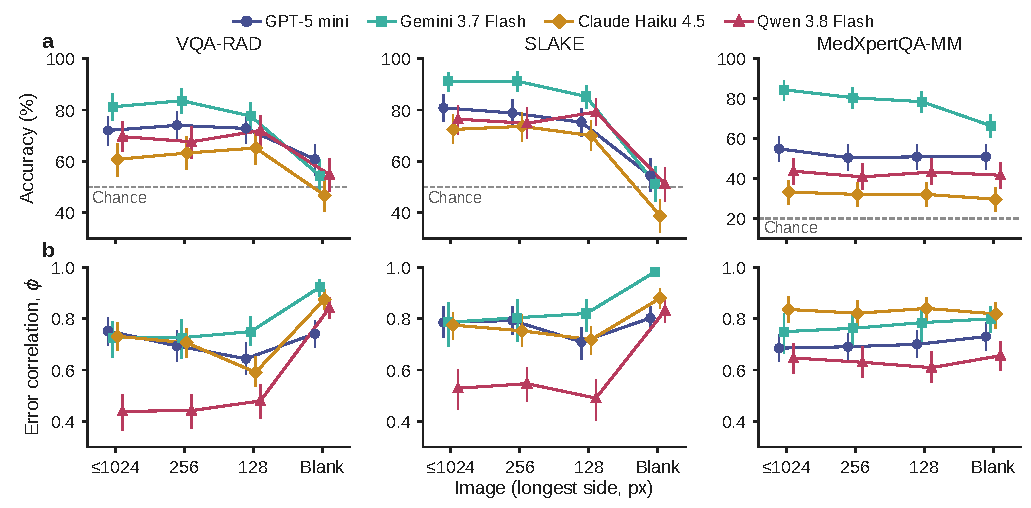
\includegraphics[width=\textwidth]{figures/supp_resolution.pdf}
\caption{\textbf{Reduced resolution changes error correlation in different directions across models.} (a) Single-agent accuracy and (b) error correlation $\phi$ of the Independent MAS across image conditions. Columns show VQA-RAD, SLAKE and MedXpertQA-MM, with 250 items each. Labels $\leq1024$, 256 and 128 cap the longest image side in pixels; Blank denotes a uniform gray image of unchanged dimensions. Lines join adjacent conditions. Dashed lines mark chance accuracy; vertical intervals are item-bootstrap 95\% CIs. Model colors as in Fig.~1.}
\label{fig:supp-resolution}
\end{figure*}

\begin{figure*}[!htbp]
\centering
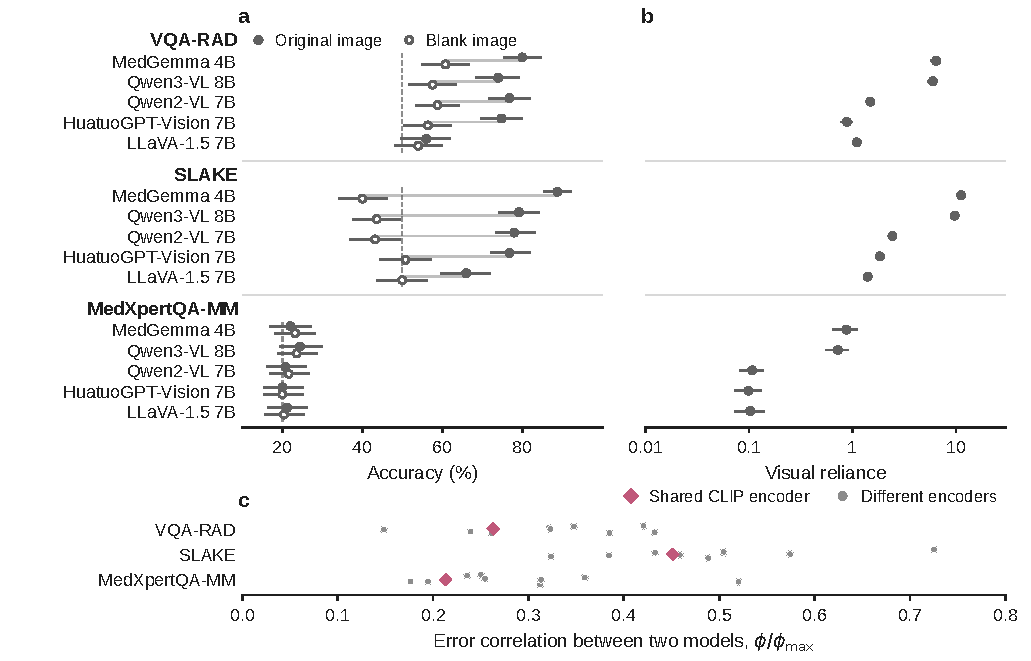
\includegraphics[width=\textwidth]{figures/supp_openweight.pdf}
\caption{\textbf{Open-weight probes show visual reliance without sampling.} Each model used one forward pass per item on VQA-RAD, SLAKE and MedXpertQA-MM, with 250 items each. (a) Accuracy with the original image (filled) and blank image (open); dashed vertical lines mark chance. (b) Visual reliance on a log scale: absolute change in log-odds of yes on binary items, and Kullback--Leibler divergence from original-image to blank-image probabilities on MedXpertQA-MM. Points are means with item-bootstrap 95\% CIs. Dark gray markers in (a,b) identify the labeled open-weight models. (c) Between-model error correlation divided by its maximum given the marginal error rates, $\phi/\phi_{\max}$. Rose diamonds identify HuatuoGPT-Vision 7B and LLaVA-1.5 7B, which share the CLIP ViT-L/14-336 encoder; gray circles identify pairs with different encoders.}
\label{fig:supp-openweight}
\end{figure*}

\clearpage
\twocolumn
\section{Text-only clinical questions}\label{sec:supp-text}

An unpublished companion analysis evaluated language-model agents on text-only clinical questions. The data sets were MedQA, MedAgentsBench and the text set of MedXpertQA~\cite{jin2021medqa,medagentsbench,zuo2025medxpertqa}. The 8 models were Claude Haiku 4.5, Claude Sonnet 5, DeepSeek V4 Flash, Gemini 3.5 Flash Lite, Gemini 3.7 Flash, GPT-4.1 nano, GPT-5 mini and GPT-5 nano. They answered as single agents and in multi-agent systems with specialty roles. The 340 configurations comprised 96 Independent, 96 Centralized, 96 Decentralized and 52 Hybrid systems, with architecture names from Kim et al.~\cite{kim2026scaling}.

Initial-answer error correlation in the companion analysis was within the imaging range. Across the 288 Independent, Centralized and Decentralized configurations with 3 to 9 agents, mean initial-answer $\phi$ was 0.758. These architectures shared initial answers and had identical initial-answer correlations by design. With 9 agents, $\phi$ was 0.762 and $N_{\mathrm{eff}}$ was 1.27.

Debate increased error correlation in the companion Decentralized systems. Across the 96 configurations, mean $\phi$ was 0.758 (SD 0.117) before debate and 0.990 (SD 0.010) after debate. After debate, $N_{\mathrm{eff}}$ was 1.01.


\end{document}
